\chapter{WebRTC Trust and Security Architecture}
\label{security}

\begin{quote}
\textit{
Information security aims at protecting the confidentiality, integrity, and availability of an information.
These objectives are referred to as the CIA triad and are often associated with additional security objectives such as non-repudiation, authenticity, and privacy.
Our research questions are centred on the idea of building a security and trust model for WebRTC.
This chapter is an introduction to the techniques, algorithms, and protocols securing WebRTC and forming the context of our thesis.
Firstly we introduce the WebRTC architecture and specifications in Section~\ref{sec:webrtc}.
Then we present an overview of the concepts accomplishing practical security on the Web in Section~\ref{sec:websecurity} and later focus on the protocols used to secure a WebRTC communication in Section~\ref{sec:webrtcid}.
We also introduce the concept of trust and present the WebRTC trust model in Section~\ref{sec:trustintro}.
Even if the content of a communication is sufficiently secure, the attacker's knowledge that a communication happened may also be a risk for the user.
In Section~\ref{sec:privacy}, we explain privacy in the context of the Web and in particular the privacy considerations of the WebRTC specification.
Finally, we present some signalling architecture that could be deployed by WebRTC services in Section~\ref{sec:voip}.
WebRTC does not specify a signalling architecture, but these have an important impact on the underlying trust and security properties.
}
\end{quote}
\glsresetall
%%%%%%%%%%%%%%%%%%%%%%%%%%%%%%%%%%%%%%%%%%%%%%%%%%%%%%
%%%%%%        WEBRTC 
%%%%%%%%%%%%%%%%%%%%%%%%%%%%%%%%%%%%%%%%%%%%%%%%%%%%%%
\section{WebRTC Overview}
\label{sec:webrtc}
%\subsection{Overview}
WebRTC is a standardisation effort for interoperable real-time communication in the Web, in line with the specifications of HTML5 technologies.
This set of specifications aims to provide for dynamic webpages\footnote{Dynamic HTML is the generic name for the set of techniques used by a webpage in order to modify itself. It is now more often referred to as a JavaScript/HTML/CSS page.}, running in a compatible browser, and suitably authorized by the user, with the capability to set up audio, video, or data communications.
The main use-cases are audio conferencing, e-commerce support, and personal or enterprise communications.
But other use-cases are also envisioned such as gaming or file sharing. 
Due to the ease of deploying a WebRTC service: a simple web server is enough, it is expected to see the emergence of a larger number of WebRTC enabled websites.

The three main tracks for WebRTC are a set of dedicated protocol profiles defined by the \gls{ietf}~\cite{I-D.ietf-rtcweb-overview}, and two JavaScript \gls{api} specified by the \gls{w3c} for WebRTC session management~\cite{w3c:webrtc} and for audio and video media capture~\cite{w3c:mediacapture}.
These specifications work in conjunction so that ``for all options and features of the protocol specification, it should be clear which \gls{api} calls to make to exercise that option or feature; similarly, for any sequence of \gls{api} calls, it should be clear which protocol options and features will be invoked''~\cite{I-D.ietf-rtcweb-overview}.
Although the endpoints targeted by the \gls{api} are web browser implementing WebRTC, it is also possible to use non-browser WebRTC endpoints.
These endpoints conform to the protocol specification but not to the WebRTC \gls{api}.
For instance, such endpoints may be a native library in C++ offering WebRTC call functionality to an application.

Figure~\ref{fig:webrtcbrowser} presents the components of the WebRTC browser model and their interactions.
The design of WebRTC does not assume that the browser should provide every functionality required by telephone or conference services.
Instead, the browser only offers functions required for a web application to implement such services.
Hence why the only vital interfaces are the RTC \gls{api} and the protocols for browser-to-browser communication.
A typical WebRTC communication setup is presented in Figure~\ref{fig:webrtcsig}.
The Media path represents the browser-to-browser communication path over which media and data channels are established.
Signalling is the communication between WebRTC endpoints establishing, managing, and controlling the media path.
The signalling path generally involves one or more signalling server to serve as a rendezvous point. 
The mechanisms and architectures for client-server and eventually inter-server signalling are out of scope of the WebRTC specification.
We present examples of such architectures in Section~\ref{sec:voip}.

\begin{figure}
\centering
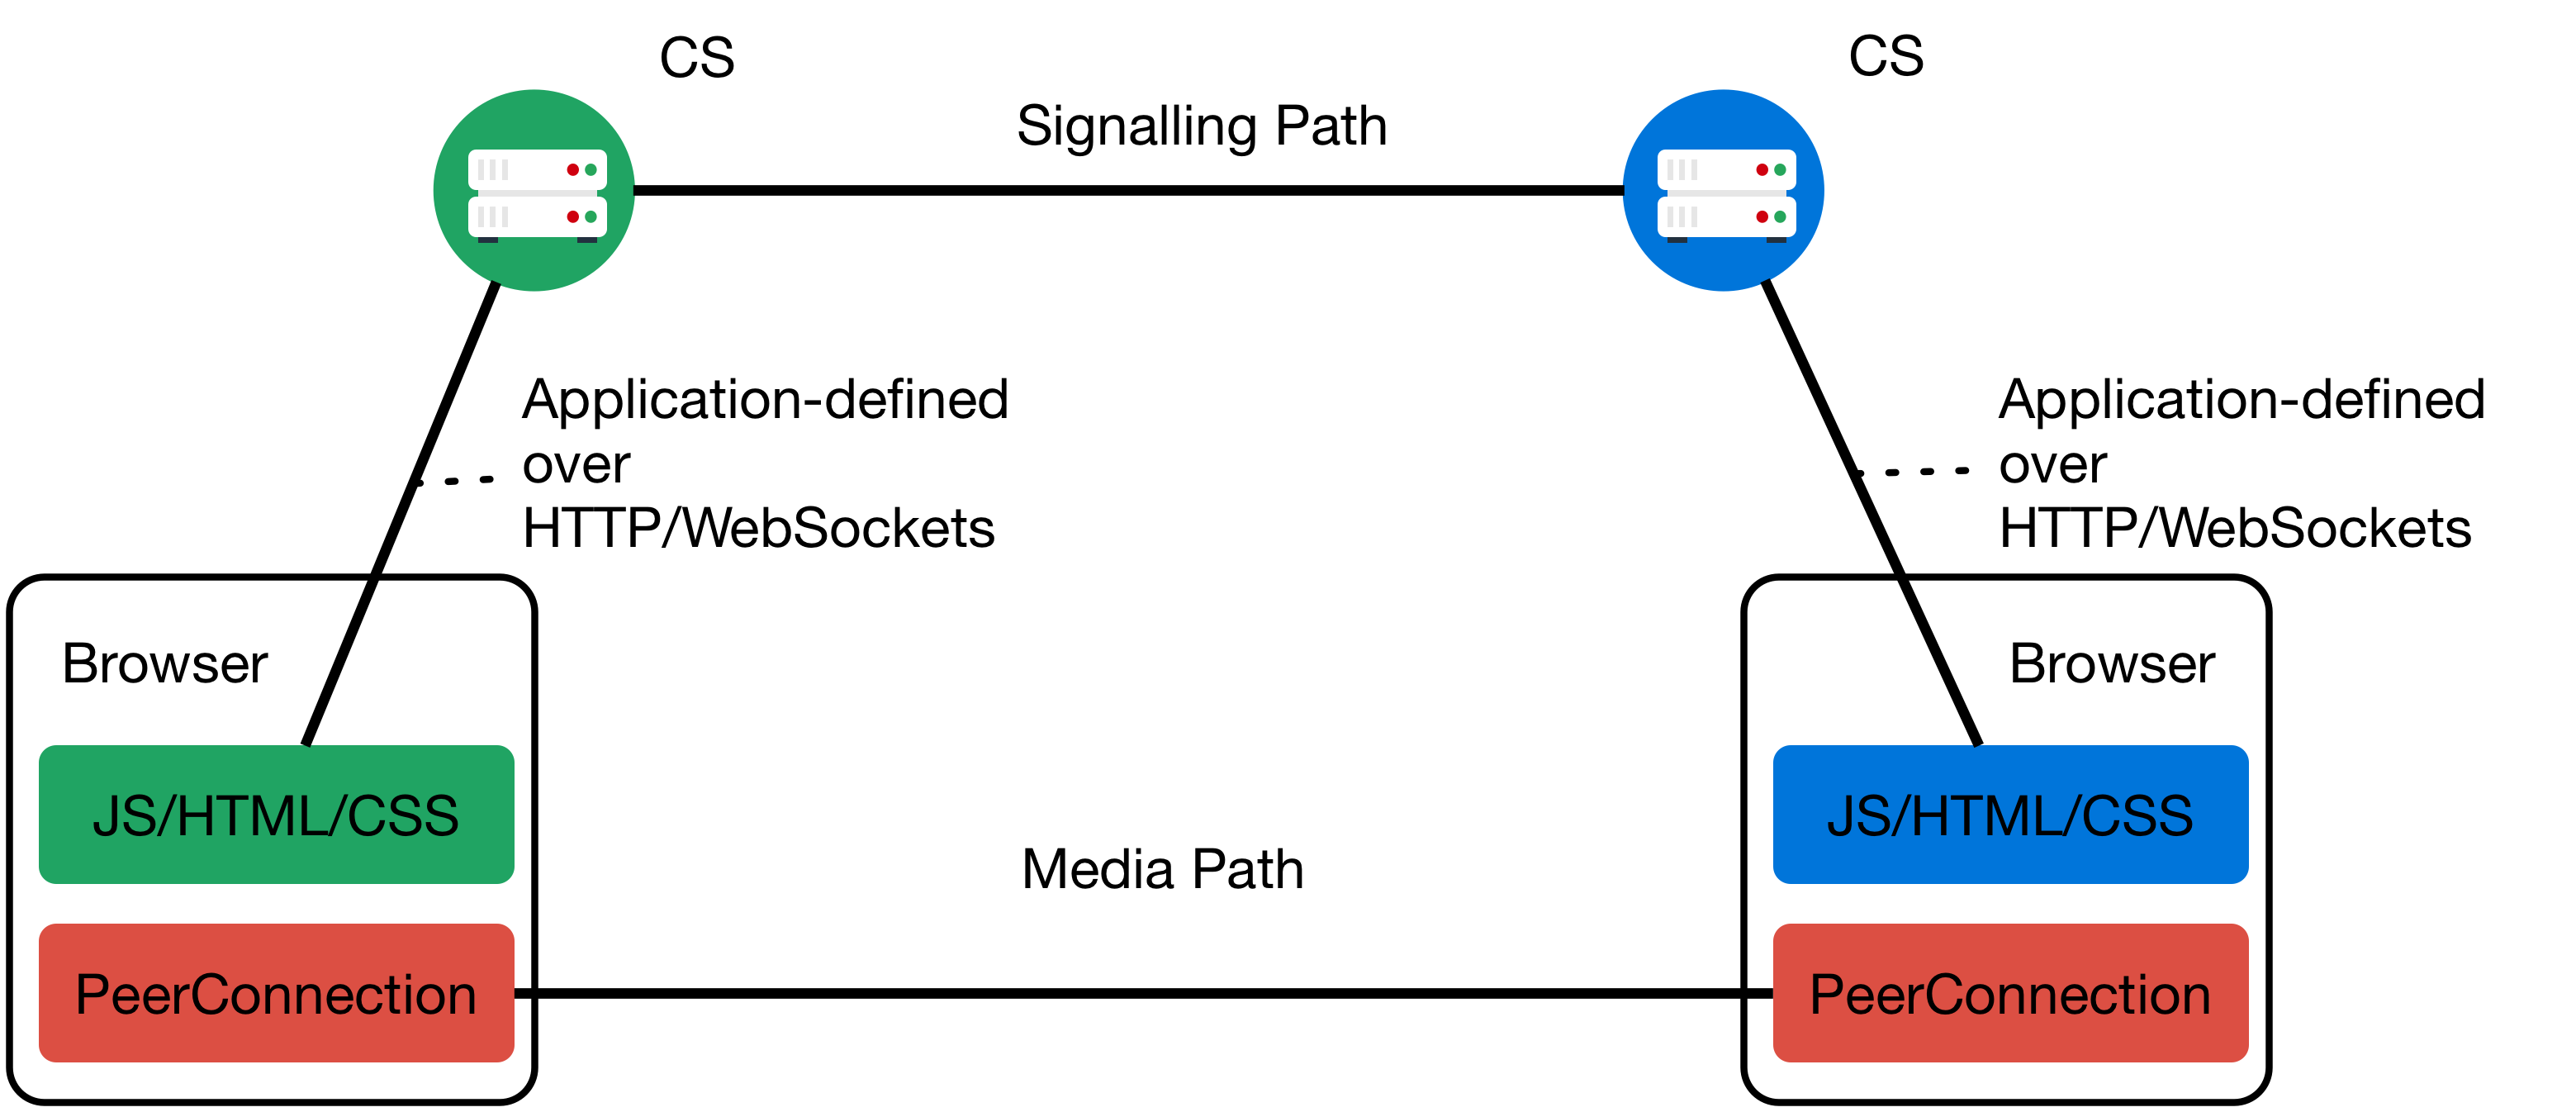
\includegraphics[width=.9\textwidth]{images/webrtcDeployment}
\caption{WebRTC deployment with two browser endpoints and two signalling servers~\cite{I-D.ietf-rtcweb-overview}.}
\label{fig:webrtcsig}
\end{figure}


\marginpar{
\captionsetup{type=figure}
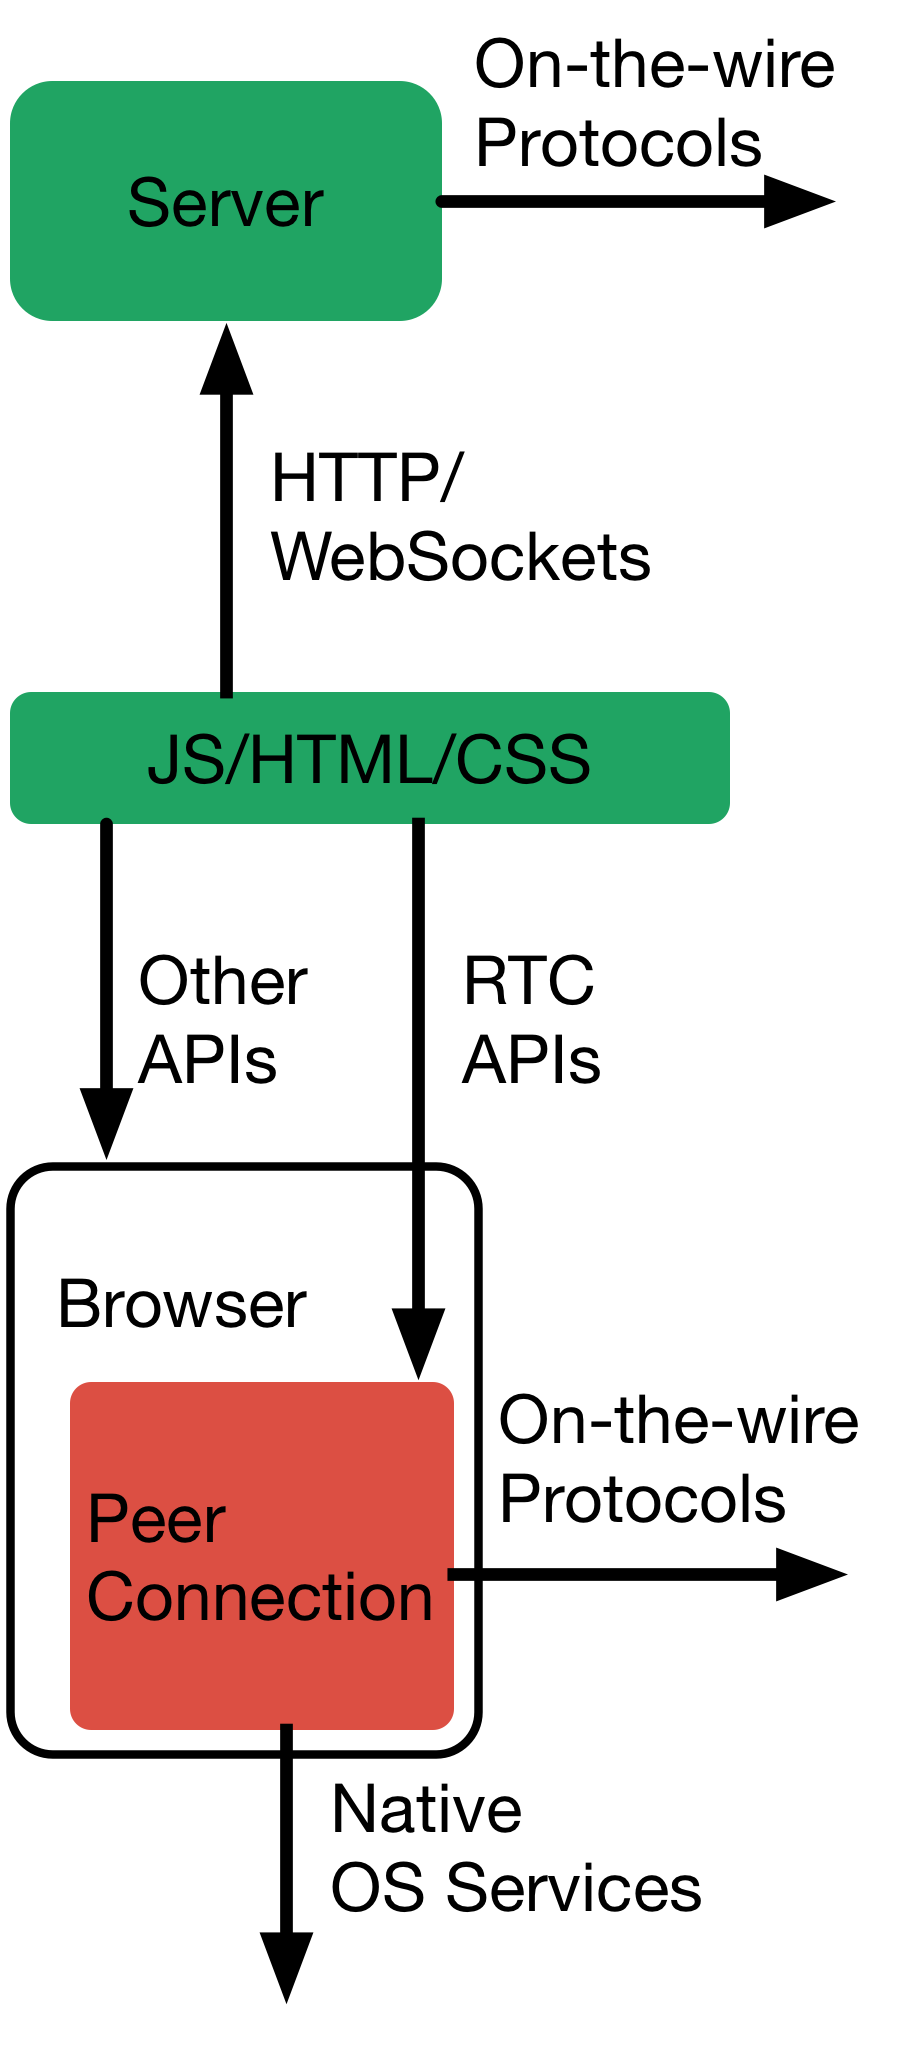
\includegraphics[width=\marginparwidth]{images/webrtcEndpoint}
\caption{WebRTC browser endpoint model~\cite{I-D.ietf-rtcweb-overview}.}
\label{fig:webrtcbrowser}
}


The main interface exposed by the WebRTC \gls{api} is the RTCPeerConnection~\cite{w3c:webrtc}.
It exposes functions to the webpage's JavaScript allowing it to manage the WebRTC session and signalling.
The \gls{jsep} \gls{ietf} draft~\cite{I-D.ietf-rtcweb-jsep} describes how the RTCPeerConnection is used.
\gls{jsep} permits the establishment and control of a WebRTC session through the exchange of session description messages, in a simple offer/answer negotiation mechanism.
When an offer/answer exchange is required, the initiating endpoint calls the \texttt{createOffer()} function. 
The resulting offer is installed as a local configuration, using \texttt{setLocalDescription()}, and transmitted on the signalling path.
When received, the offer is used as a remote configuration, with the \texttt{setRemoteDescription()} interface.
Finally, the process is reversed: the receiver generates an answer, applies it as a local configuration, and sends it.
On receiving the answer, the initiator installs it as a remote description, completing the initial setup.

Session description messages use the \gls{sdp}~\cite{RFC2327} syntax, as presented in Figure~\ref{fig:sdpsyntax}.
The \gls{sdp} syntax defines a list of parameters, identified by type letters and belonging to one of the description levels: the session description level, the time description level, and one or more media description level. 
The set of type letters is quite small and not extensible, however, extensions are possible through the use of \texttt{a=} attribute lines.

\begin{figure}
\begin{verbatim}
Session description
        v=  (protocol version)
        o=  (owner/creator and session identifier).
        s=  (session name)
        i=* (session information)
        u=* (URI of description)
        e=* (email address)
        p=* (phone number)
        c=* (connection information - not required if included in all media)
        b=* (bandwidth information)
        One or more time descriptions (see below)
        z=* (time zone adjustments)
        k=* (encryption key)
        a=* (zero or more session attribute lines)
        Zero or more media descriptions (see below)

Time description
        t=  (time the session is active)
        r=* (zero or more repeat times)

Media description
        m=  (media name and transport address)
        i=* (media title)
        c=* (connection information - optional if included at session-level)
        b=* (bandwidth information)
        k=* (encryption key)
        a=* (zero or more media attribute lines)
\end{verbatim}
\caption{Session Description Protocol syntax}
\label{fig:sdpsyntax}
\end{figure}
% after audio
%a=sendrecv
%a=fmtp:109 maxplaybackrate=48000;stereo=1;useinbandfec=1
%a=fmtp:101 0-15
%a=ice-pwd:cf1b0f7d3182718ee580de9a5bc68645
%a=ice-ufrag:495d215b
%a=mid:sdparta_0
%a=msid:{0e832fa8-b782-0549-9e9e-3a071487d5c6} 
%    {979b603a-395e-2941-aa8d-e2bc0ddb0033}
%a=rtcp-mux
%a=rtpmap:109 opus/48000/2
%a=rtpmap:101 telephone-event/8000
%a=setup:active
%a=ssrc:2196327089 cname:{17ce3841-2445-ba43-a3a7-60e428f22d43}

Figure~\ref{fig:sdpexample} shows an example of a (shortened) \gls{sdp} message for a WebRTC session.
It is an \gls{sdp} answer for a session with audio and video channels, respectively identified as \texttt{sdparta\_0} and \texttt{sdparta\_1}.
Declaration of these channels starts with a \texttt{m} line specifying the channel type, \eg \texttt{m=audio}.
In the \gls{sdp} offer/answer negotiation, peers have to agree on various parameters, for example, audio and video codecs.
In order to conduct the negotiation, an offer includes multiple supported parameters.
If compatible, the answerer accepts these parameters by including them in his answer.
Preceeding this example, the original offer proposed five codecs for the audio channel: \texttt{opus}, \texttt{telephone-event}, \texttt{G722}, \texttt{PCMU}, and \texttt{PCMA}.
Only two, \texttt{opus} and \texttt{telephone-event}, are included in the answer and thus accepted by the answerer.


\begin{figure}
\begin{verbatim}
v=0
o=mozilla...THIS_IS_SDPARTA-54.0.1 5897145307417630851 0 IN IP4 0.0.0.0
[...]
a=fingerprint:sha-256 33:B1:D7:4B:29:29:29:AA:87:01:47:B3:59:41:[...]5D
a=group:BUNDLE sdparta_0 sdparta_1
a=ice-options:trickle
a=msid-semantic:WMS *

m=audio 29188 UDP/TLS/RTP/SAVPF 109 101
c=IN IP4 74.125.39.43
a=mid:sdparta_0
a=candidate:0 1 UDP 2122252543 131.254.67.174 54163 typ host
[...]
a=candidate:20 1 UDP 8331263 74.125.39.43 29188 typ relay [...]
a=rtpmap:109 opus/48000/2
a=rtpmap:101 telephone-event/8000
[...]

m=video 29188 UDP/TLS/RTP/SAVPF 121
c=IN IP4 74.125.39.43
a=mid:sdparta_1
[...]
\end{verbatim}
\caption{Example of a SDP message (answer)}
\label{fig:sdpexample}
\end{figure}

In order to efficiently communicate in a \gls{p2p} fashion, peers use the \gls{ice}~\cite{RFC5245} to find which of their network interfaces are able to see each other.
Indeed, a computer may be connected to different networks through different interfaces.
In the \gls{ice} protocol, peers collect candidate addresses and exchange them during the \gls{sdp} negotiation in \texttt{a=candidate} attributes.
Each pair of local and remote candidates are then tested to find potential matching interfaces. 
In some situations, for example behind a \gls{nat}, a peer may not know his publicly visible address. 
\gls{stun}~\cite{RFC5389} is a client-server protocol used by a client to discover the binding between his source address and his reflexive transport address\footnote{NAT modify the source or destination of packets going through them. The reflexive transport address is the public \gls{ip} address and port created by the \gls{nat} closest to the \gls{stun} server.}.
\gls{stun} is a tool that may not work in some configuration, in particular, if both peers are behind \gls{nat} routers with endpoint-dependant-mechanisms for address attribution.
In that case, a relay can be setup using the \gls{turn}~\cite{RFC5766} extension to \gls{stun}.
Once ICE checks have completed, both peers can set up their secure channels.



%%%%%%%%%%%%%%%%%%%%%%%%%%%%%%%%%%%%%%%%%%%%%%%%%%%%%%
%%%%%%        WEB SECURITY
%%%%%%%%%%%%%%%%%%%%%%%%%%%%%%%%%%%%%%%%%%%%%%%%%%%%%%

\section{Security on the Web}
\label{sec:websecurity}
The World Wide Web, or more commonly the Web, is one of the many applications of the Internet.
It allows to retrieve and manipulate resources hosted by a server and referencing other resources by hypertext links.
The Web is built on a client-server model, and the most common type of client is, of course, the web browser.
Web clients are often referred to as user-agents, particularly in web specifications.

The set of protocols and specifications forming the Web are mainly defined by two standardisation bodies.
Languages such as HTML and CSS, protocols such as the \gls{http}, and web \gls{api} such as WebRTC \gls{api} are standardised by the \gls{w3c}~\cite{W3CStandard, W3CAPI}.
As the Web is built on the Internet, the \gls{ietf} contributes to protocol specifications which are then used in the context of the Web.
The \gls{ecma} is also an important actor as it standardises the ECMAScript programming language, better known under the name of Mozilla's implementation: JavaScript.
Browser makers, as the implementors of the most used web clients, are also central to the definitions, evolutions, and adoptions of web specifications.
The most important browser makers are Google (Chrome), Mozilla (Firefox), Microsoft (Edge/IE), and Apple (Safari). Figure~\ref{fig:w3schools} gives a rough indication of the balance of power between these main four browsers.
If a feature is not implemented or removed from one of the popular browsers it will soon be abandoned by websites.
Yet, implementing the full standard specifications is a daunting task and browsers, although regularly updated, often offer incomplete support for some features.
Keeping up with particular features and implementations from each browser is a complex task for website developers.
A common technique is to conditionally use \textit{shims} or \textit{polyfills}, adapter code that abstract browsers' implementations under a single interface.


\marginpar{
\captionsetup{type=figure}
\centering
\begin{tikzpicture}
\begin{axis}[
    ybar=0pt,
    ytick={0,25,50,75},
    axis y line*=none,
    axis x line*=none,
    tick label style={font=\footnotesize},
    legend style={font=\footnotesize},
    label style={font=\footnotesize},
    width=\marginparwidth,
    bar width=2.5mm,
    xtick=data,
    %xmin=-1,
    %xmax=2,    
    yticklabels={0\%, 25\%, 50\%, 75\%},
    xticklabels={w3school.com,gs.statcounter.com},
    xticklabel style={rotate=45},
    ymin=0,
    area legend,
    legend style={at={(1,1)},anchor=south east},
    y=.5mm,
    enlarge x limits={abs=0.5}
    %enlargelimits=false
    %enlarge y limits={abs=0.},
]
\addplot[ybar,matred,fill=matred] coordinates{(0,3.3)(1,14.2)};
\addplot[ybar,matblue,fill=matblue] coordinates{(0,4.6)(1,3.6)};
\addplot[ybar,matorange,fill=matorange] coordinates{(0,13.3)(1,6)};
\addplot[ybar,matgreen,fill=matgreen] coordinates{(0,76.3)(1,55.7)};

\legend{Safari, Edge/IE, Firefox, Chrome}
\end{axis}  
\end{tikzpicture}
\caption{Percentage of recorded browsers visiting \protect\url{w3schools.com} and \protect\url{amiunique.org} in June 2017.}
\label{fig:w3schools}
}

\subsection{The Trusted Computing Base}
\label{sec:tcb}
The \gls{tcb} is the set of hardware and software on which the security of a system relies upon.
In a correct implementation of a \gls{tcb}, if a part of the \gls{tcb} is compromised, then the whole system's security may be at risk.
However a compromised component not part of the \gls{tcb} should not present a risk to the security of the system in general or to any other components in particular.
While from an \gls{os} point of view the browser is just an application outside of the \gls{tcb}, in the context of the Web the browser is a central part of the \gls{tcb}. 

In other words, the browser can actually be considered as the \gls{os} of the Web.
Indeed, it is responsible for downloading and running client web application, while exposing resources and services through web \gls{api}.
As other \gls{os}, the browser is also responsible for maintaining applications isolation.

\subsection{The Same Origin Policy}
For web applications, isolation relies on the concept of origin and the same-origin policy~\cite{RFC6454}.
An origin is a protection domain regrouping \gls{uri}~\cite{RFC3986} sharing the same triple of scheme, host, and port.
Two pages from different origins are isolated and cannot share resources, such as variables or cookies.
However, communication is still possible using the postMessage \gls{api}.
This interface allows pages from different origins to exchange scoped message and cloned variables.

\begin{figure}
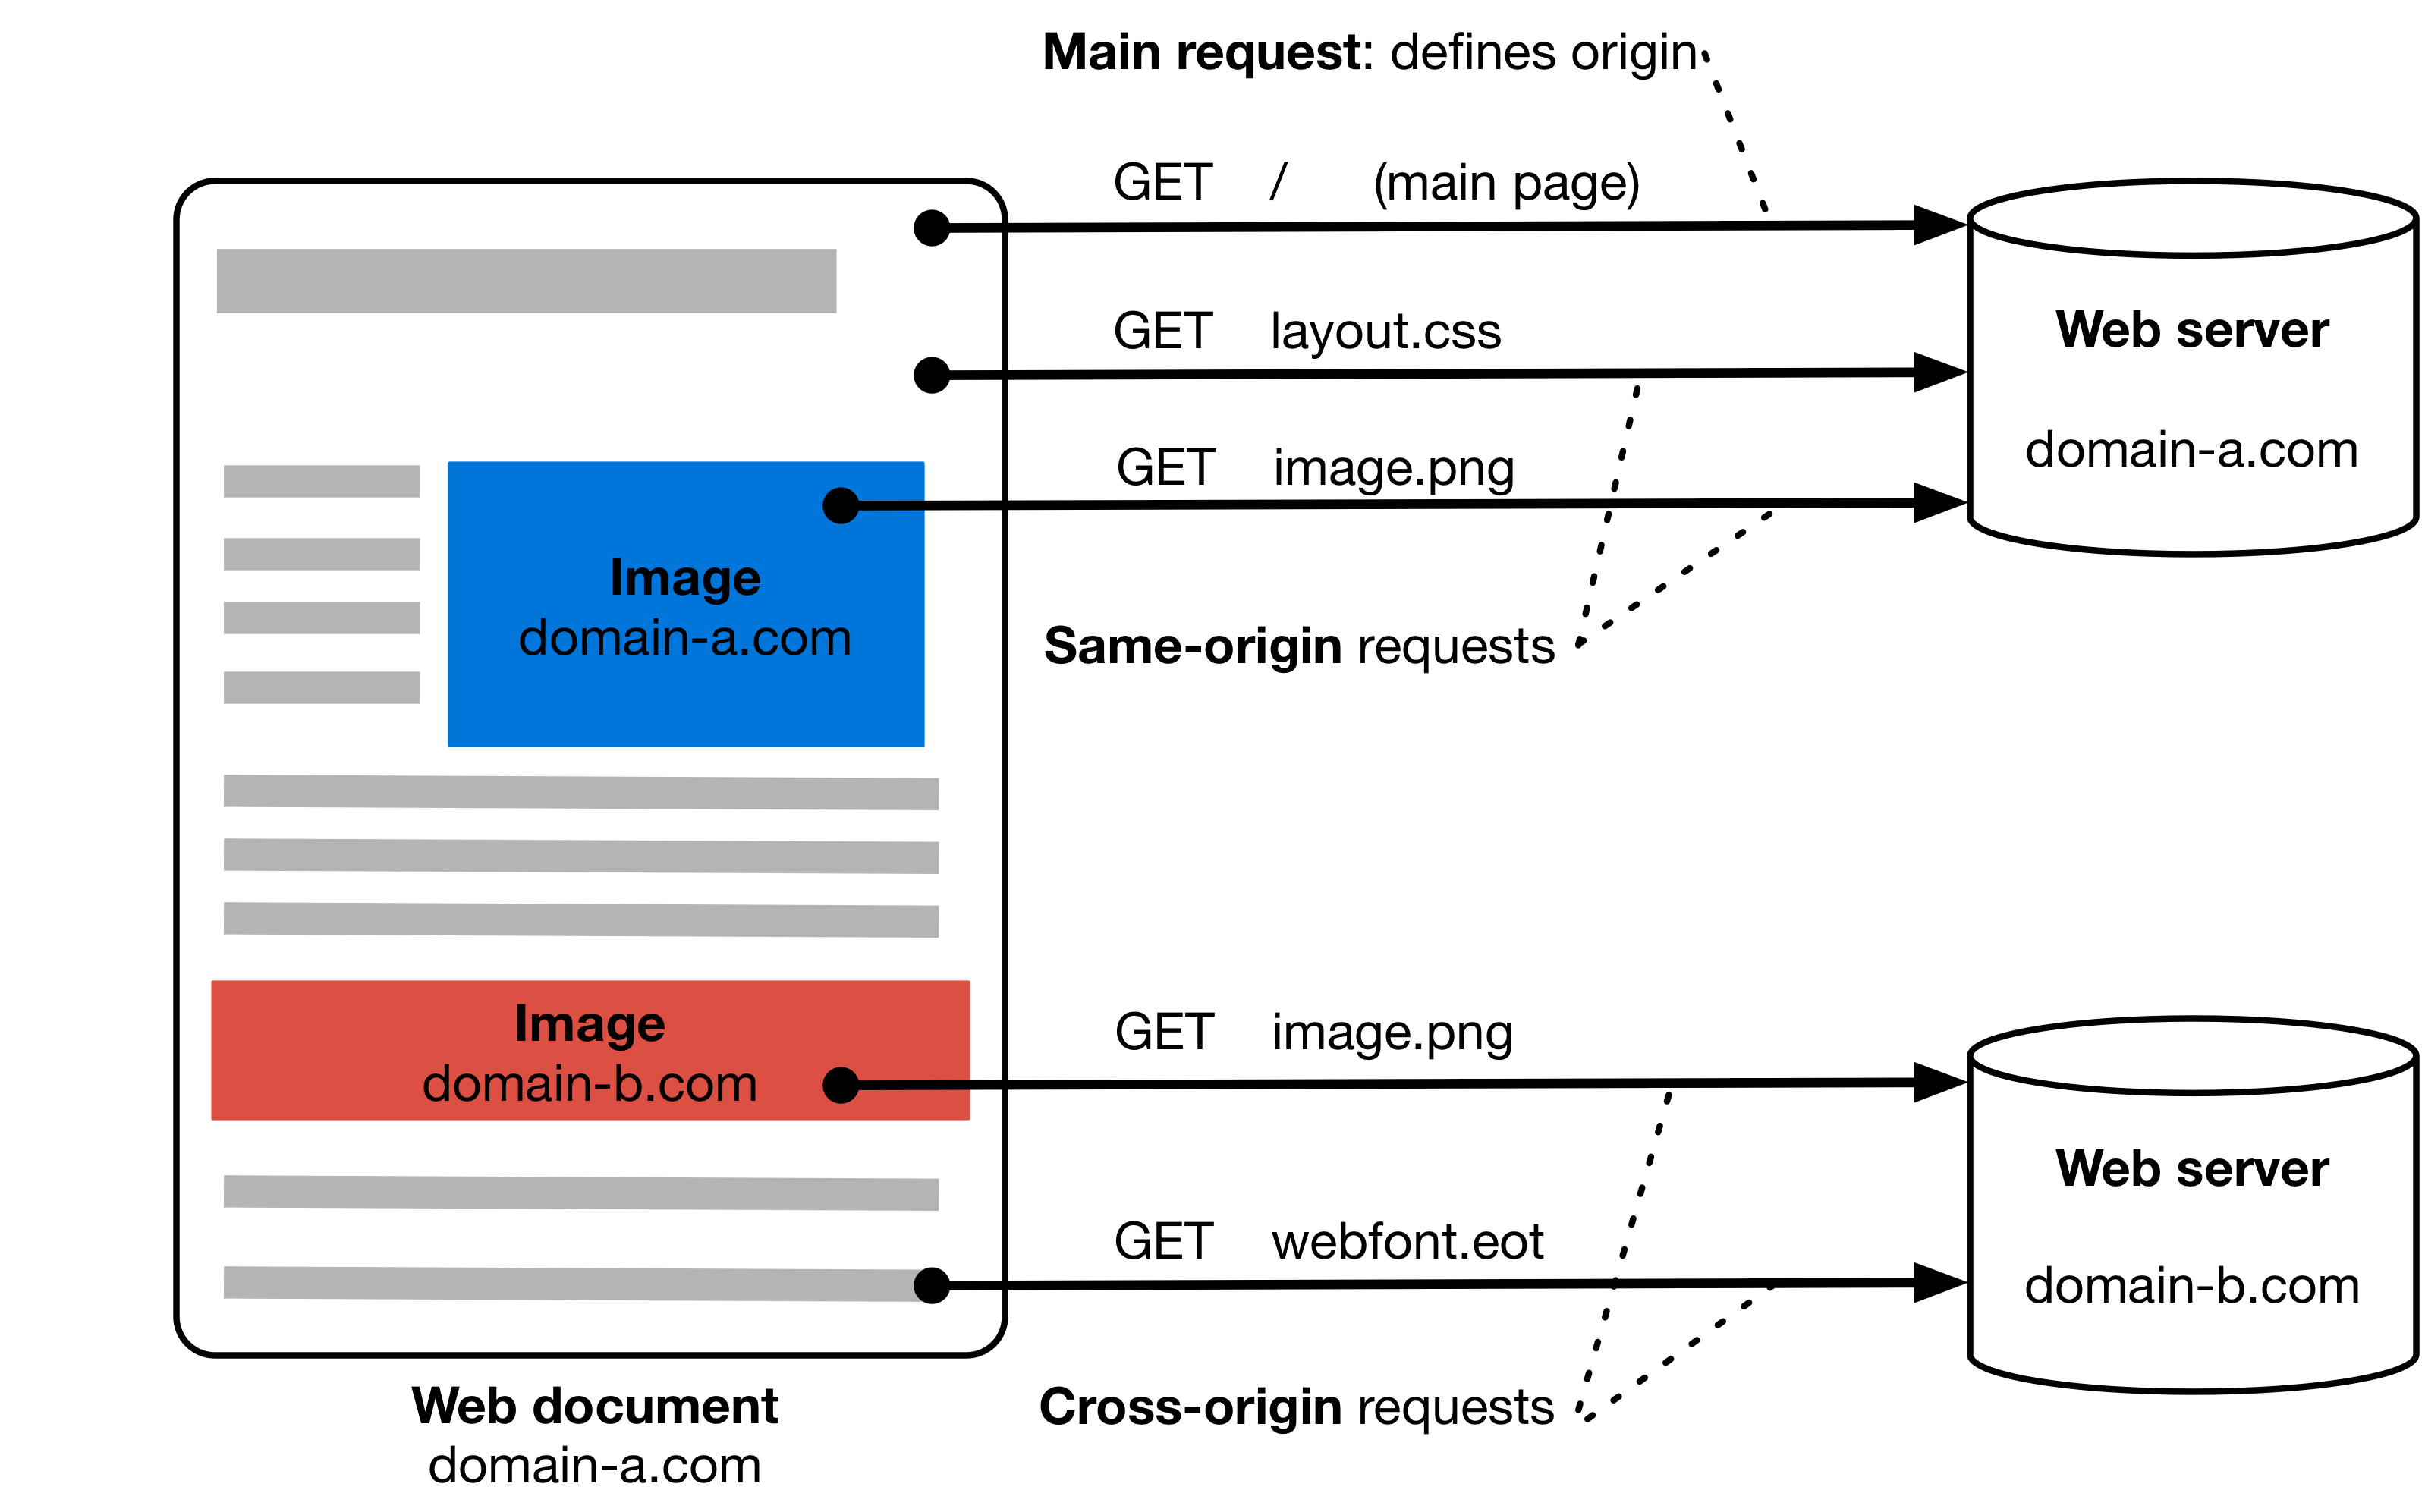
\includegraphics[width=\textwidth]{images/CORS}
\caption[Cross-site Request Example]{Cross-site request example. The HTML page from \protect\url{domain-a.com} requests resources from \protect\url{domain-a.com} and \protect\url{domain-b.com}. Requests for \protect\url{domain-a.com} are same-origin and always allowed. Requests for \protect\url{domain-b.com} are cross-origin and requires valid CORS headers and CSP directives. Example taken from \protect\url{developer.mozilla.org}.}
\label{fig:cors}
\end{figure}

A web application can also embed contents such as scripts or images from other origins. 
Figure~\ref{fig:cors} shows an example of a webpage with content loaded from two different domains.
Cross-origin content may enable vulnerabilities in a webpage as it enables the coexistence of two origins in a single security-context.
\gls{xss} and others code injection attacks exploit the user's trust in a webpage.
This kind of privilege escalation attack allows a malicious script to gain access to sensitive session information from the security context of the main origin.
One way for a webpage to prevent \gls{xss} is to define whitelisted origins through the use of \gls{csp} directives~\cite{9524886}.
This ensures that only trusted content can be loaded and executed by the web application.
Unlike \gls{xss} attacks, \gls{csrf} attacks exploit a web application's trust in a user's authentication to issue commands in place of the user.
To issue a \gls{csrf} attack a malicious webpage visited by the user executes an illegitimate \gls{http} request on the vulnerable server.
The request may, for instance, be triggered by loading a link inside an HTML image element or the execution of a JavaScript fetch request.
Supposing that the user is authenticated on the vulnerable application the illegitimate request inherits from this authentication, for instance through a session cookie.
Web applications may deter \gls{csrf} attack by enforcing the same-origin policy for some of their exposed \gls{http} interface.
This can be achieved by setting unique and unpredictable csrf-token cookie on the client side, or by defining \gls{cors}~\cite{RFC6454} headers on \gls{http} responses.
In both types of attacks, \gls{csrf} and \gls{xss}, the browser is responsible for correctly applying policies defined by web applications in order to protect the user.

Web-based protocols may require the discovery of policy or configuration information through metadata.
In order to avoid collisions with existing resources but also prevent impersonation on self-hosting services, \gls{rfc} 5785~\cite{RFC5785} defines well-known \gls{uri}.
A well-known \gls{uri} is a \gls{uri} whose path components starts with \texttt{/.well-known/}.
Specifications often define resources located under a well-known \gls{uri} and assume that they are under control of the host.


\subsection{The HyperText Transfer Protocol Secure}
\label{sec:https}
\glsreset{http}
\glsreset{tls}
\glsreset{https}
The \gls{http}~\cite{RFC2616} is an Internet application layer protocol~\cite{RFC1122} developed to access and modify web resources.
It offers several methods to send resource requests from a client to a server.
The two main ones are GET which is used to retrieve a resource, and POST which is used to send data to the server for creating or updating a resource. 
Responses to \gls{http} requests are made of a status code and an eventual body containing the actual response, \eg a file or an object.
For instance, the status code 200 means that the request is successful while the set of 300 codes indicates a redirection.

\gls{https}~\cite{RFC2818} is the combination of the \gls{http} and \gls{tls}~\cite{RFC5246} protocols\footnote{Note that as HTTP is not considered secure, HTTP and HTTPS page from the same domain are not considered to be from the same origin.}.
\gls{tls} enables authentication and secure communication between a client and server\footnote{Although client authentication is also possible with TLS, it is not much used and often limited to server-server interactions or other particular use cases.}. 
To authenticate itself to a client a server must provide a signed and valid certificate containing, in particular, his public key, his domain name, and the certification authority which issued the certificate.
After the client validated the certificates, it uses the public key to communicate a secret session key to the server initiating a secure communication between both parties.

Certification authorities are the entities responsible for issuing and signing certificates.
There exist four types of \gls{https} certificates ranging from self-signed certificates to Extended Validation certificates.
These types differ from the verification conducted by certification authority, their costs, and the way they are displayed by browsers.
Although there is debate whether Organisation Validation certificates offer more guarantees as Domain Validation certificates.
Some Extended Validation certificates are integrated by browser makers within their browser installation packages.
These are often referred to as root certificates as they do not depend on other certificates.
It is the responsibility of the browser makers to select trustworthy certification authority for providing root certificates.

In addition to initialising trust chains, the responsibility of the browser is to provide security information to the user when they connect to a website.
This is usually done by displaying a colour coded indications of the page security level in the address bar and in-context warning such as in Figure~\ref{fig:httpssecurity}.
Mixed contents such as an insecure login forms are also taken into account to determine the security level.
However, if the certificate is invalid the page is automatically blocked by the browser.
While this effectively deters attacks, users usually only see false alarms~\cite{herley2009so} which could, in turn, have the effect of lowering their vigilance.

Browser makers are currently pushing \gls{https} and advocating for a fully encrypted Web.
For instance, Firefox indicated that they will advertise \gls{http} site similarly to bad certificate~\cite{mozillasecurityblog2017communicating}. 
A full \gls{https} web would lower the trust of users in \gls{http} websites, and force those site to finally adopt \gls{https}.
This objective is made possible thanks to automated \gls{ca} such as Let's Encrypt which operates the \gls{acme} protocol.
Let's Encrypt aims at drastically reducing the complexity and cost of certificate deployment by avoiding manual operations, a major barrier for the multitude of small websites.
Ultimately, the usage of \gls{https} is not a proof of trustworthiness of the website itself but only that the control of its domain name was verified to some extent and that secure communication is in place.

\marginpar{
\captionsetup{type=figure}
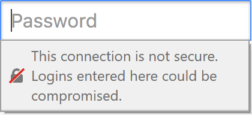
\includegraphics[width=\marginparwidth]{images/firefox_warning}\\\\
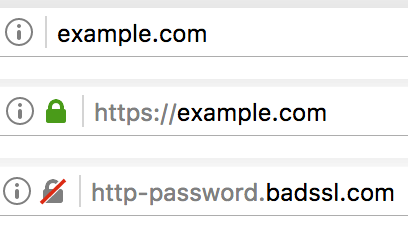
\includegraphics[width=\marginparwidth]{images/httpslevel}
\caption[Web Browser Security Indications]{Security indications for HTTP, HTTPS and insecure password form on Firefox. The HTTP indicator will soon be replaced by a warning similar to the example shown here.}
\label{fig:httpssecurity}
}

\subsection{Public Key Cryptography}
\label{sec:pubkey}
This section introduces the notion and usages of public key cryptography, a corner-stone of the security of the Web.
This technique allows to sign, authenticate, and secure messages exchanged by two peers without the need to share a common secret key.
Public key cryptography is used in the certificate infrastructure deployed by browsers and \gls{ca} for \gls{https}, but also in the WebRTC security protocols, and in authentication delegation protocols.


In 1976 Diffie and Hellman published the concept of public key cryptography, also called asymmetric cryptography.
The race for such an algorithm was won by Ron Rivest, Adi Shamir, and Leonard Adleman with the publication of the famous RSA algorithm.
In symmetric cryptography, the same key is used to encrypt and decrypt the message. 
This is, for instance, the case with Caesar's cypher where the key is the number of shifts to apply in order to encrypt a plaintext message, but also the number of opposite shift to decrypt the message. 
Conversely, public key cryptography protocols use two keys.
The secret key is randomly generated while the public key is derived from the secret key, both forming a key pair.
As knowledge of the public key does not allow to retrieve the private key, the public key can be shared freely.
We do not go into details on the specific cryptography mechanisms and algorithms but focus on the use cases made possible by asymmetric cryptography.

In order to bind an identity to a key pair, a \gls{ca} issues a digital certificate.
These certificates contain information about the public key, the signing algorithm, the owner's identity, and the \gls{ca}.
Certificates may also refer to the \gls{ca}'s own certificate until a trusted root certificate is reached forming a chain of trust.
X.509 certificates, one of the most used standards for digital certificates, contain several fields describing the certificate itself, the issuer, and the subject.
An example is given in Figure~\ref{fig:x509}.
Another way to issue certificates is to participate in a web of trust where members respectively sign their keys during key exchange party.
OpenPGP~\cite{RFC4880} is the most widely used web of trust standard, particularly for signing emails.

\begin{figure}
\begin{tabular}{@{}ll@{}}\toprule\toprule
   \textbf{Subject} & \\
   Common Name & energyq.idp.rethink.orange-labs.fr \\\midrule
   \textbf{Subject's Public Key} & \\
   Public Key Algorithm & PKCS \#1 RSA Encryption \\
   Public Key & c5 44 1c 33 79 bf e5 [...] c9 26 a4 e3 5e 4e 6d\\\midrule
   \textbf{Issuer} & \\
   Common Name & Let's Encrypt Authority X3 \\\midrule
   \textbf{Period of Validity} & \\
   Begins On & 31 mai 2017 \\
   Expires On &  29 ao�t 2017\\\midrule
   \textbf{Fingerprints} & \\
   Signature Algorithm & PKCS \#1 SHA-256 With RSA Encryption \\
   SHA-256 Fingerprint &  77:21:3C:64:0A:ED:E3:AD:0F:82:03:6D:9B:45:66:B4:\\ & D0:28:D8:04:9E:F3:41:C1:C7:A5:EA:57:BB:A0:34:1D\\\bottomrule
   \hline
\end{tabular}
\caption[X.509 Certificate]{Extract of a X.509 certificate issued by Let's Encrypt to energyq.idp.rethink.orange-labs.fr. }
\label{fig:x509}
\end{figure}

\begin{figure}[H]
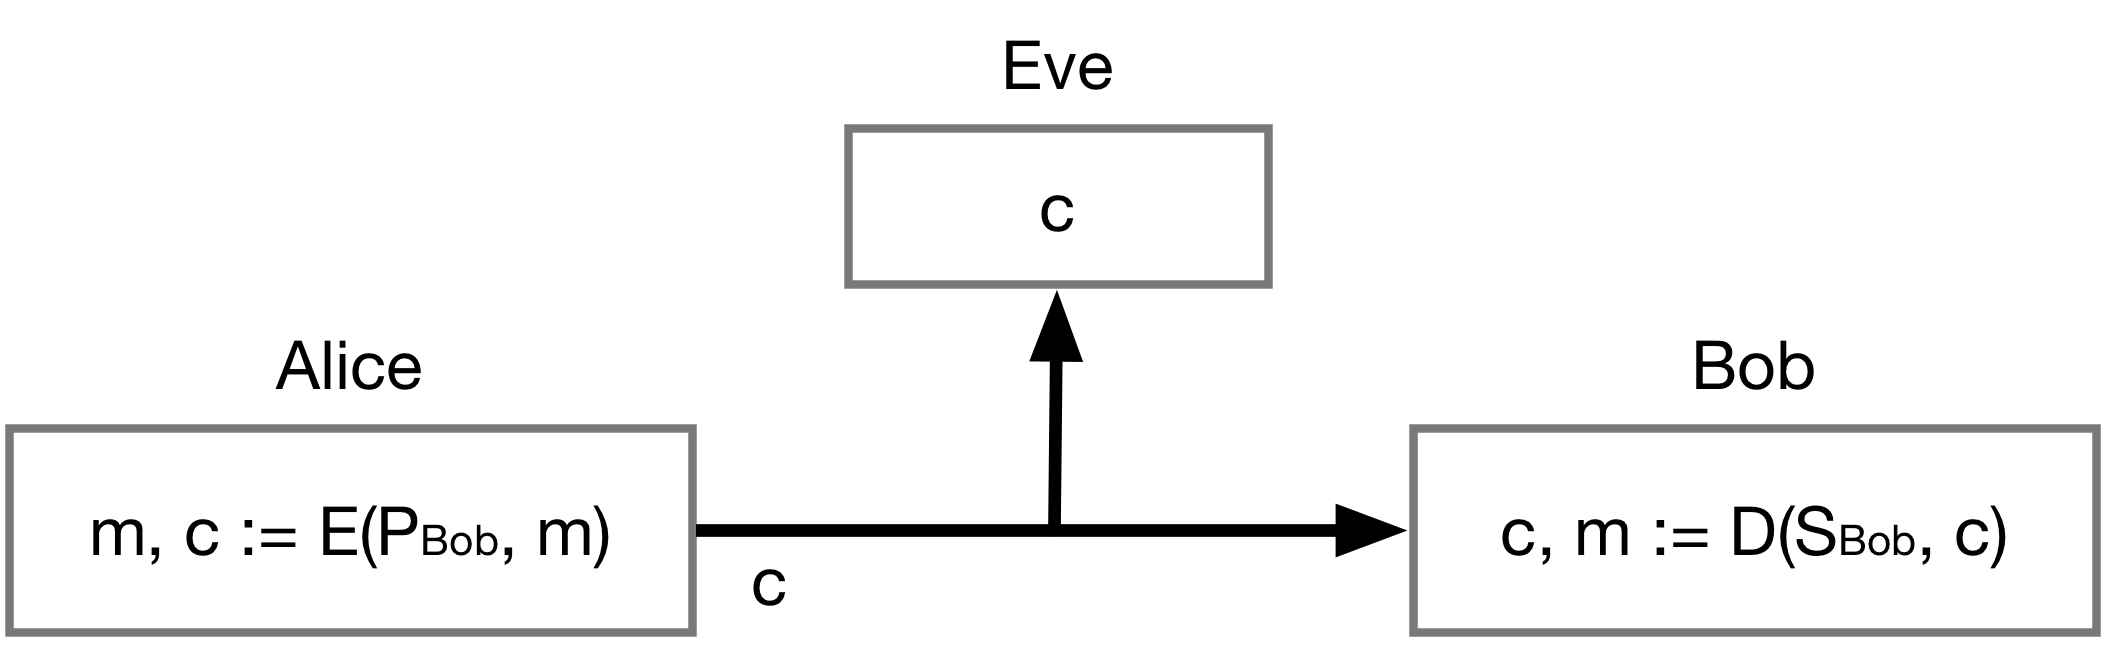
\includegraphics[width=.7\textwidth]{images/encrypt}
\caption{Public-key encryption of $m$ from Alice to Bob~\cite{ferguson2011cryptography}.}
\label{fig:symenc}
\end{figure}

In the public key encryption scenario (Figure~\ref{fig:symenc}), Alice wants to send an encrypted message $m$ so that it is only readable by Bob, the intended recipient.
Bob possesses a key pair $(P_{Bob}, S_{Bob})$ and publishes its public key.
Alice then uses this public key to encrypt the message and send the cyphertext to Bob.
On receiving the encrypted cyphertext, Bob uses its secret key to decrypt the message.
While the attacker Eve could not read the cyphertext, it could still intercept the message and modify it. 
Confidentiality is ensured, but encryption does not prove message integrity nor the sender's authenticity.


\begin{figure}[H]
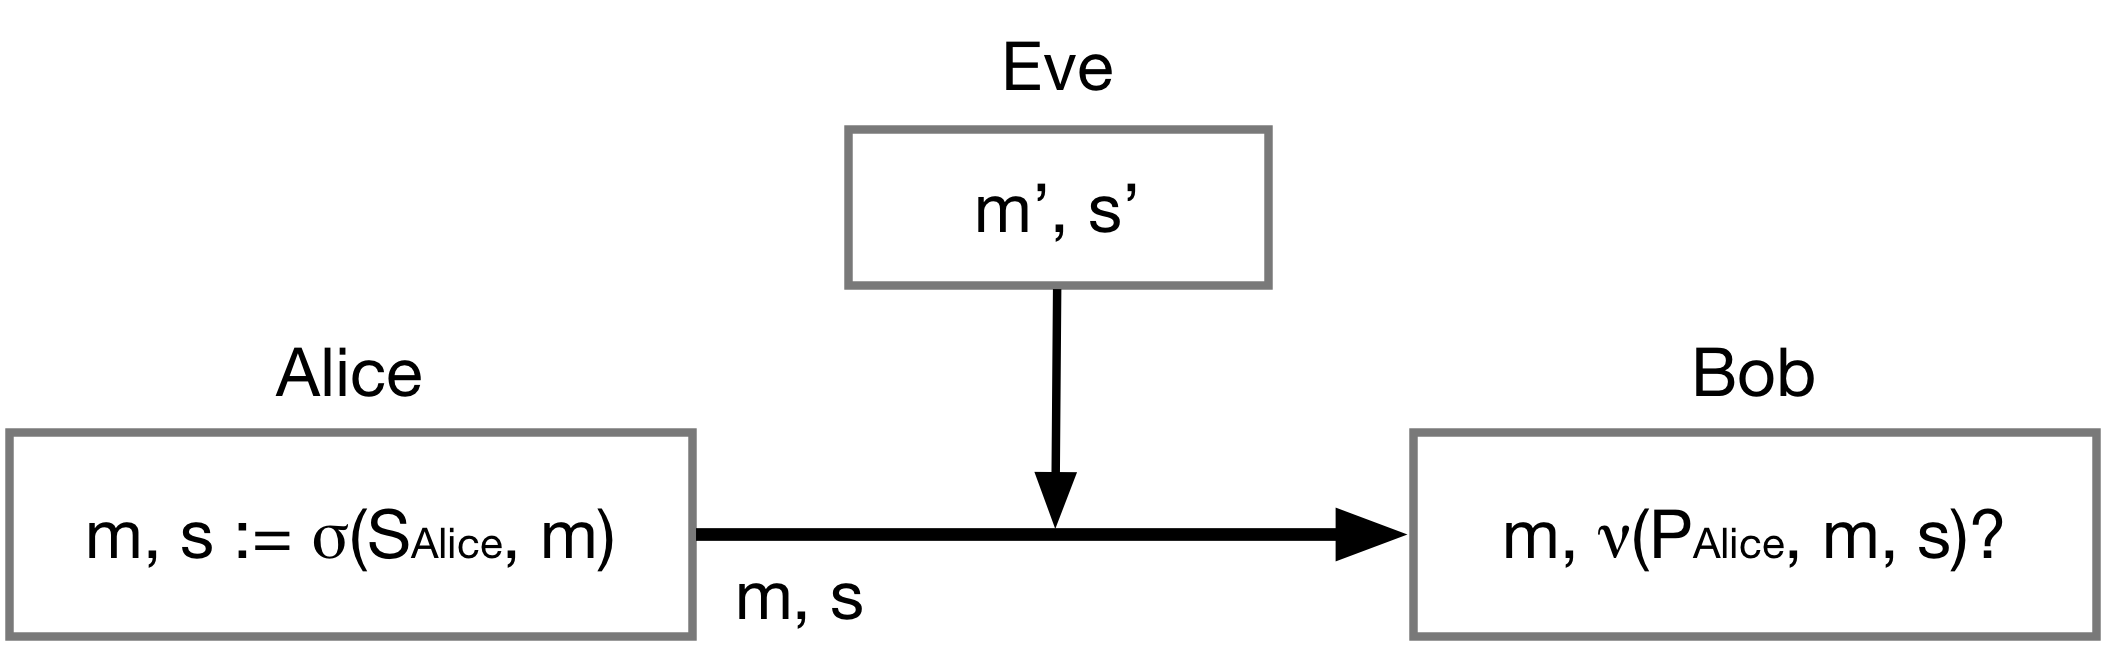
\includegraphics[width=.7\textwidth]{images/signature}
\caption{Public-key signature of a message $m$ from Alice to Bob~\cite{ferguson2011cryptography}.}
\label{fig:symsig}
\end{figure}

In the signature scenario (Figure~\ref{fig:symsig}), Alice possesses a key pair $(P_{Alice}, S_{Alice})$ and publishes its public key.
In order to sign a message $m$, Alice uses a signing algorithm with the private key and the plain text as a parameter to produce a tag, \ie the signature $s$.
She then sends both plain text and signature to the recipient.
The signature algorithm is often associated with a cryptographic hash function, a one-way function mapping the message to a fixed size string.
In this case, the signature is applied on the resulting hash, also called a digest.
By verifying the signature with the public key and comparing it to the message, or the message's digest, the receiver is then able to verify the integrity of the received message.
Only the holder of the secret key could have produced the signature.
If the key pair is bound to the sender's identity, for instance with a certificate containing the sender's name, the receiver also verifies the authenticity of the message.

Achieving both confidentiality and integrity is possible if both parties publish their respective public keys.
To do so the sender would sign the message with its own private key and then encrypt both message and signature with the other party's public key.
Using asymmetric encryption is, however, a computationally heavy operation compared to symmetric encryption. 
In order to solve this problem, public key cryptography is used to establish a symmetric session key.
Such key exchange scheme is often referred to as a Diffie-Hellman exchange.

A cypher suite is a standardised configuration of cryptographic algorithms and options meant to serve as a toolbox for establishing a secure communication.
In \gls{tls}, a cypher suite would define the key exchange algorithm, the bulk encryption algorithm, the signature algorithm and the relevant key size to be used.
Prior to starting the negotiation, both peer would make a hand-shake to compare their respective available cypher suite and find a common ground.
Figure~\ref{fig:cyphersuit} shows the cypher suit used on \url{idp.energyq.rethink.orange-labs.fr} with Firefox.

\marginpar{
\captionsetup{type=figure}

\footnotesize{\textbf{TLS\_ECDHE\_RSA\_\\WITH\_AES256\_GCM\_\\SHA384}}
\caption[Cypher Suit Example]{This cypher suit defines ECDHE as the key exchange mechanism, RSA as the authentication mechanism, AES\_256\_GCM as the symmetric encryption algorithm, and SHA384 as the digest algorithm.}
\label{fig:cyphersuit}
}


%%%%%%%%%%%%%%%%%%%%%%%%%%%%%%%%%%%%%%%%%%%%%%%%%%%%%%
%%%%%%        WEBRTC SECURITY
%%%%%%%%%%%%%%%%%%%%%%%%%%%%%%%%%%%%%%%%%%%%%%%%%%%%%%
\section{WebRTC Security}
\label{sec:webrtcid}

While the signalling path is secured as any other client-server connection on the Web.
The media path serves for real-time media communications and as such uses different protocols.
Figure~\ref{fig:stack} shows the protocol stack for the WebRTC signalling and media path.
WebRTC mandates the use of secure media channels\footnote{A consistent decision with the direction for HTTPS everywhere.}~\cite{I-D.ietf-rtcweb-security-arch}.
In this section we present the protocols protecting confidentiality, integrity, and availability of the media channel.
The WebRTC security architecture also introduces an optional identity path to let users verify their peer's authenticity.
We give definitions related to user authenticity in Section~\ref{sec:authn} and present the WebRTC Identity Path in Section~\ref{sec:webrtcidpath}.
We also give an overview of some alternative key management protocols in Section~\ref{sec:keymanagement}.

\begin{figure}
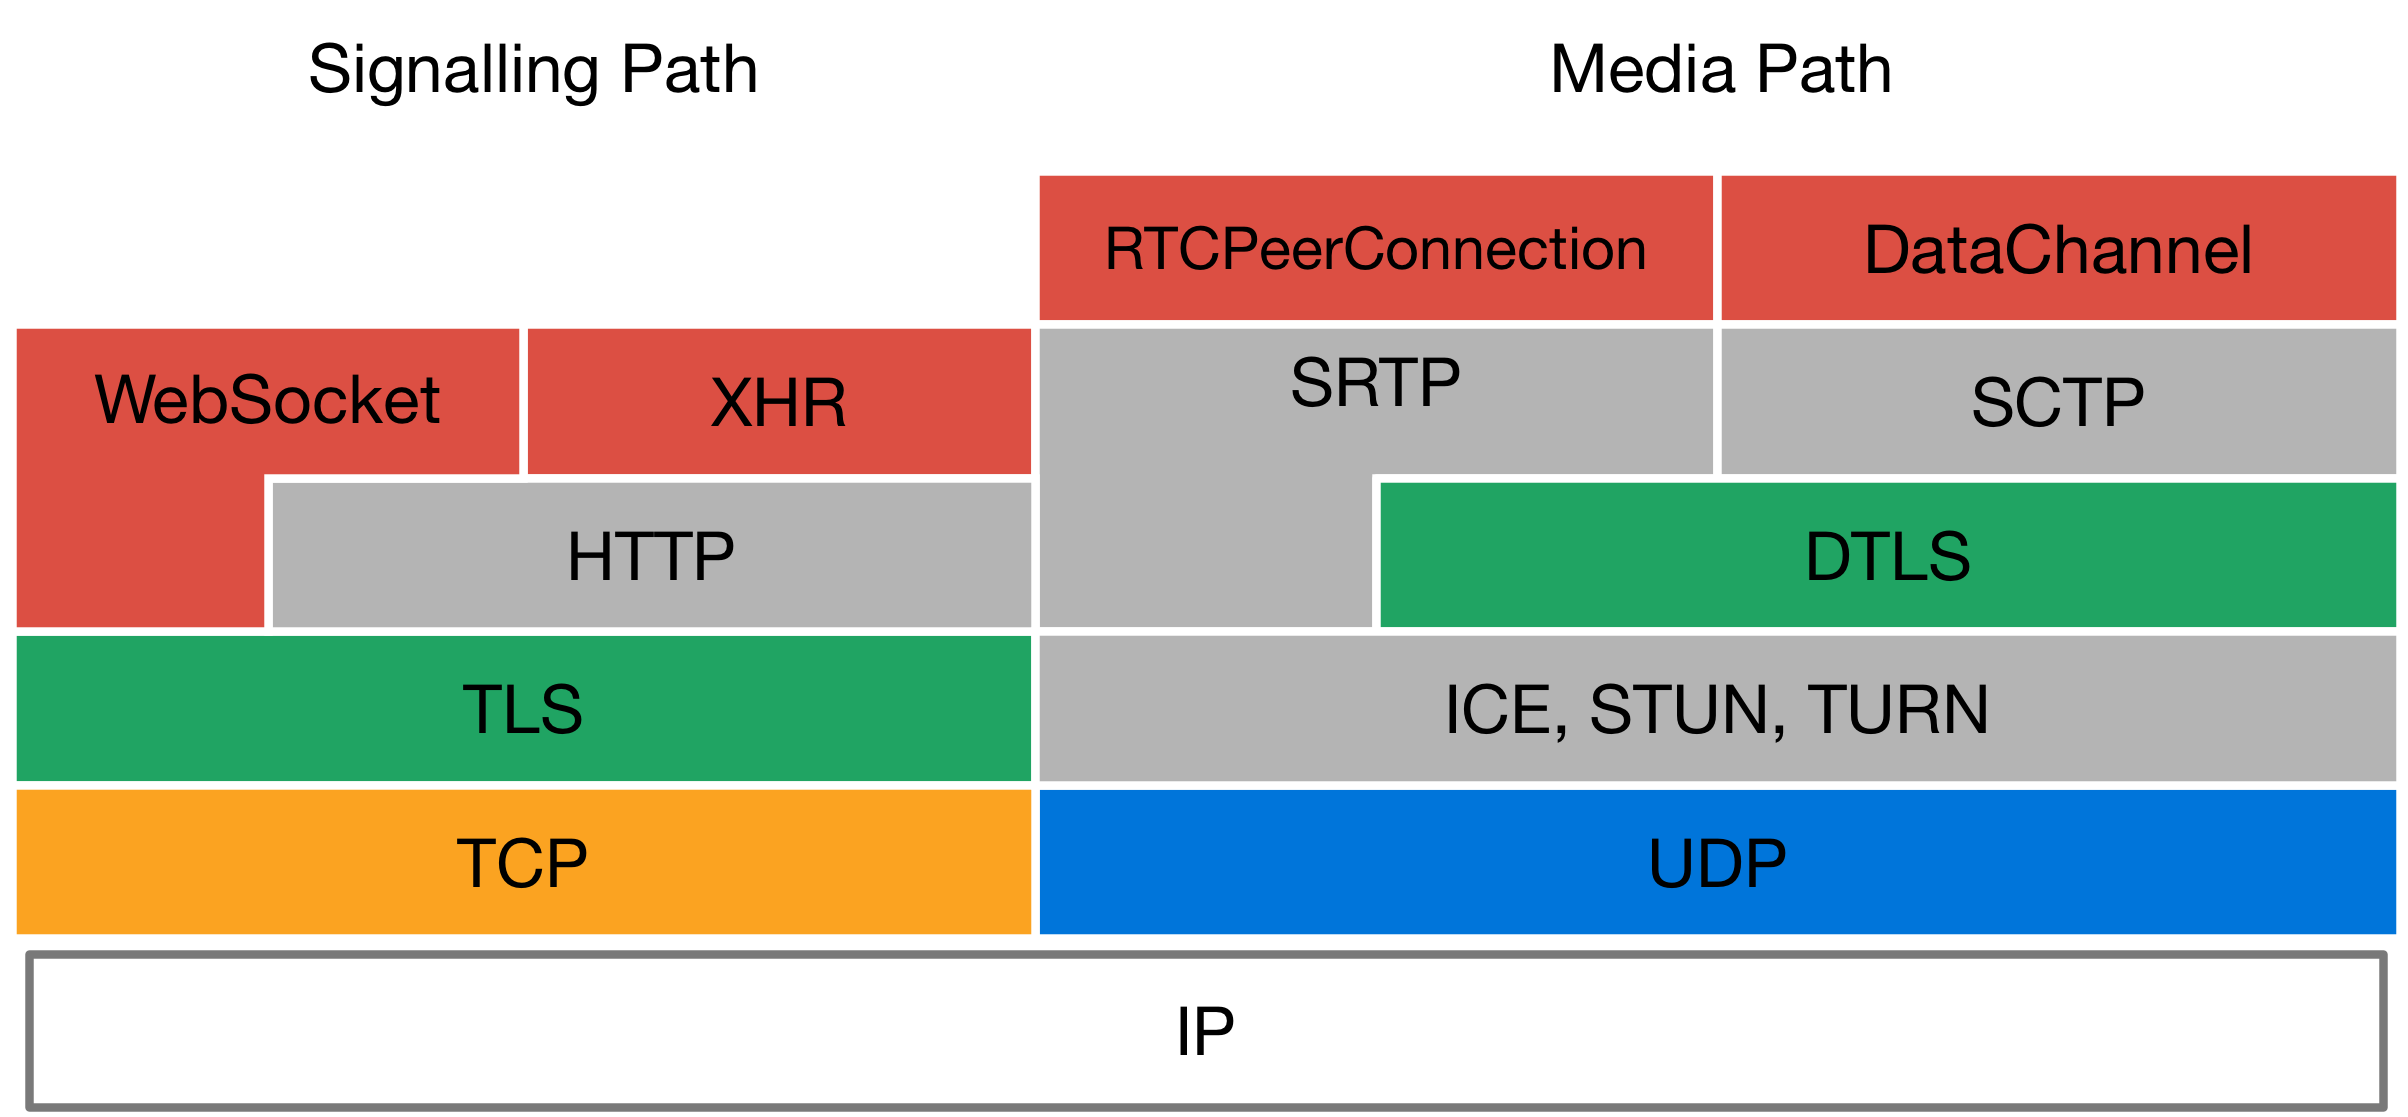
\includegraphics[width=.8\textwidth]{images/webrtcStack}
\caption{WebRTC Protocol Stack~\cite{HPBN}.}
\label{fig:stack}
\end{figure}

\subsection{Confidentiality and Integrity of the Media Path}
The media path is a \gls{p2p} connection between two WebRTC endpoints.
This path allows both the setup of media streams offered by the Media Capture and Streams \gls{api} or data channels from the RTCDataChannel \gls{api}.

\glsreset{srtp}\glsreset{rtp}\glsreset{rtcp}\glsreset{srtp}
Media streams are transported over the \gls{srtp}~\cite{RFC3711}, a secure profile for the \gls{rtp}~\cite{RFC3550} and \gls{rtcp} ``which can provide confidentiality, message authentication, and replay protection''.
Usually, the \gls{rtp} protocol (and \gls{srtp}) is carried over the \gls{udp}~\cite{RFC768} as real-time media streams are time-sensitive\footnote{Contrary to the \gls{tcp}~\cite{RFC793}, UDP does not guarantees the delivery, ordering, or duplicating of its packets and avoids the overhead of such guarantees.}.
As \gls{srtp} does not offer key management functionality, it must rely on another key management protocol.
The preferred and default protocol for \gls{srtp} key management is the \gls{dtlssrtp}~\cite{RFC5763} which must be offered by any WebRTC implementation.
\gls{dtls}~\cite{RFC6347} is an adaptation of \gls{tls} to datagram transport protocols.
\gls{dtlssrtp}~\cite{RFC5764} is ``a \gls{srtp} extension for \gls{dtls} that combines the performance and encryption flexibility benefits of \gls{srtp} with the flexibility and convenience of \gls{dtls}-integrated key and association management''.
\gls{dtlssrtp} can thus be seen as a \gls{dtls} optimisation for \gls{rtp}.
On the other hand, data channels use the \gls{sctp}\footnote{SCTP can be configured to provide similar features to UDP or TCP.}~\cite{RFC4960} and are secured by \gls{dtls} only.

In order to exchange their public keys and setup a session key, peers proceed to a \gls{dtls} handshake over the media path by exchanging certificates.
Contrary to server exposing certificates signed by trusted \gls{ca}, peers' certificates are self-asserted and thus untrusted.
In order to authenticate the received certificates, fingerprints of these certificates are previously exchanged over the signalling path in session level \texttt{a=fingerprint} \gls{sdp} attributes (see Figure~\ref{fig:sdpexample} for an example).
As long as the signalling path is trusted, the confidentiality and integrity of the media path is ensured.


\subsection{Availability of the Communication}
\label{sec:availability}
The main threat to availability of a WebRTC communication consists in \gls{dos} attacks, and in particular \gls{ddos}.
As WebRTC calls are programmatically controlled, a malicious software could launch multiple calls from several users to a single destination, for instance a call-center.
The consent mechanisms required by the Media Capture and Streams \gls{api} mitigate these kinds of attack using media streams.
However, data channels do not require consent before being initialised and may be used to mount \gls{ddos} attacks.
Client applications and automated WebRTC implementations, \ie call-center gateway, should implement filtering policies to detect and respond to suspicious call, \ie call without audio or video.
The WebRTC security architecture~\cite{I-D.ietf-rtcweb-security-arch} details and reference additional availability attacks against WebRTC. 

More generally, WebRTC clients may also be vulnerable to \gls{spit}, \ie the transmission of bulk unsolicited call offers.
The possibility of WebRTC spam depends on the underlying signalling architecture.
For instance an open signalling federation would be more vulnerable to \gls{spit} than a one-way call service deployed on a website.
Nonetheless, there is few doubts that in the former case a spam agent would be easy to write.
\gls{rfc}~5039~\cite{RFC5039} references solutions to \gls{spit} call for \gls{sip} that could probably be adapted to WebRTC scenarios.
One solution proposed by the RFC is to implement white and black lists to automatically accept or reject incoming calls.
However, obtaining a new identity may be quite cheap making black lists ineffective. 

Finally, a WebRTC session may be impacted by the available bandwidth on the network.
Janczukowicz \etal\cite{JanczukowiczBTB16} demonstrate that concurrent \gls{tcp} flow may have an impact on the perceived quality of a WebRTC flow under best-effort routing.
Saturating a network path could thus be used to compromise the availability of the communication.
Alternative routing mechanisms could be used to provide specialised and paid communication services with a managed quality of service.
For instance using \gls{turn} servers for routing the media path, rather than using \gls{p2p} best-effort~\cite{JanczukowiczBTF15}.
However, specialised services on the internet are criticised by some as being against the philosophy of the Net Neutrality\footnote{The french \gls{arcep} published a state of the art report on net neutrality regulations and operators practices in September 2015~\cite{ARCEPNet}.}.


\subsection{User Authenticity}
\label{sec:authn}
For users navigating the Web, authentication is a common action involving an identifier and a password.
But it may be difficult for them to explain what are the authentication inherent concepts, and what precisely is their identity.
In the following paragraphs, we define and explain the concepts of identity, identifier, credentials, and claims.
We explain what constitutes an authentication process, and what makes it secure.

A subject's \textit{identity} is a set of attributes, called claims, representing the subject in a specific scope~\cite{identityCrisis}.
As an identity is only defined for a specific scope, and a subject may exist in multiple scopes, a subject may have multiple identities.
For instance, the claims described by a subject's driver license constitutes one of his identity. 
The same subject may also have a passport and some social network accounts.
Although these identities belong to the same individual and may overlap, for instance sharing the same name and age, they are distinct identities.

Identity is often used in the sense of an identifier~\cite{identityCrisis, usercentricity06}.
This confusion is due to the fact that a name, or a public identifier in digital identity, is often used as a synonym for an identity.
In the rest of our thesis, we will clearly make the distinction to avoid confusion.

\textit{Claims} are the attributes constituting an identity.
Identity claims can describe features of a user such as his name, his age, or his address.
But claims may also be used to grant access to resources.
In that case, we talk about authorization claims.
Though some of the claims on a driver license would be describing the driver itself, \eg \texttt{name:~Bob} or \texttt{age:~30}.
Some other claims may describe the category of cars the driver is authorized to drive, \eg \texttt{cat.~A: authorized}.
On the Web, an authorization claim may allow write and read access to some data or \gls{api}.
Claims are usually uniquely identified by a URI or reserved names defined by various standards.
For instance the OpenID Connect~\cite{sakimura_openid_2014} specification defines a set of standard identity claims.
As claims can change over time, an identity may also be dynamic.

An \textit{identifier} is a claim uniquely identifying the subject in a given scope.
Identifiers may have different forms such as a pseudonym, an email address, or a random text.
A website identifies the claimed identity by looking up its records and verifying if such identifier exists. 

\textit{Authentication} is the process by which an entity proves the validity of some claims to another party.
In the most common scenario, a user authenticates by claiming his identifier.
In this case, we say that the user authenticates himself (or just authenticates if unambiguous).
In order to prove the ownership of an identifier, \ie to authenticate, the user has to present valid \textit{authentication factors}.
Contrary to identifiers, authentication factors are not necessarily unique.
Indeed, several users may, by coincidence, use the same password. 
%However, these should be resistant to common attacks, as described in Section~\ref{later subsection}.\todo{define entropy for password}

Although authentication commonly refers to proving the ownership of an identifier, it is also possible to authenticate non-identifying claims.
%Pursuing data minimization (see Section~\ref{sec:privacy}), 
For instance, to protect its privacy a user may want to claim only his age without revealing his identifier.
In order to allow for this scenario, a trusted third-party is often necessary to assert the validity of claims.
However, identification remains possible if enough claims are provided.

In the most simple case, authentication is a simple relation involving two participants.
However, for privacy, usability, or security reasons, the process may be delegated to a trusted third party.
An \gls{idp} is a trusted authority issuing and validating identity claims.
The \gls{rp} is the consumer of identity claims.
Technically, claims are requested, obtained, and validated using authentication delegation protocols.
These protocols allow the exchange of claims through security tokens.
Depending on the protocol, the \gls{rp} requests some claims to an \gls{idp} or to the subject before granting access to a service\footnote{An \gls{rp} is also commonly referred to as a Service Provider. However, we reserve this term for the context of WebRTC. Note that due to the need of authenticating users, a WebRTC Service Provider is often an \gls{rp} too.}.

Usually, the \gls{idp} is responsible for the lifecycle of an identity.
This includes the enrolment, the management, and the eventual revocation of an identity.
Before validating any claims, verifying authentication factors, and checking an identifier, the identity must first be created.
\textit{Enrolment} is the registration process used to create or update an identity.
In this situation, there are two possible stances: to define a new identity ex nihilo or to create an identity from a previously existing one, \eg by authenticating a national identity card.
In some use cases, \eg banking or communications, a server may require a user's identity to be anchored into a trusted identity.
To cater for these different needs, the \gls{aal} have been proposed by several national or regional frameworks and later standardised as ISO:29115:2013~\cite{ISO29115}.
These frameworks categorise the \gls{aal} into four roughly equivalent categories, though details may differ for historical or cultural reasons.
Hatin \etal\cite{hatin_continuous_2017} propose a mapping of these discrete levels into a continuous authentication score.
Authentication strength may also be associated with a time to live or an eroding factor applied over time.
Such authentication model shows similarity to trust models (see Section~\ref{sec:trustintro}) and current work on pervasive authentication systems further contributes to closing the gap between authentication and trust levels~\cite{hatin_continuous_2017}.

Alternatively, some servers may be satisfied to know that a user is indeed just a returning customer.
In these cases, the actual identity of the user is not that important and the server is more concerned with the authentication.
Such identity can be qualified as a declarative identity and its claims are said to be self-asserted.
Although confidence in the authenticity of such identity may be low, anchoring it into a source of reputation such as a social network may prove its trustworthiness.
Conversely, verifying that identity documents are genuine and up to date is a complex task~\cite{DBLP:conf/coria/AwalA16,DBLP:conf/iciap/SicreAF17}.

\subsection{WebRTC Identity Path}
\label{sec:webrtcidpath}
In some scenarios, users may not trust the website or the underlying communication provider on which they are making the call. 
Indeed, the signalling server may be lying about the connection authenticity and could be mounting a man-in-the-middle attack.
This type of attack, presented in Figure~\ref{fig:mitm}, allows an invisible attacker Eve to be setup in the middle of the media path between Alice and Bob by a malicious signalling server S.
When Alice sends her \gls{sdp} offer to Bob through S, the offer is instead relayed to Eve.
Eve then generates an offer to Bob and configured so that Alice's media stream is relayed to Bob.
Bob believing to be receiving a legitimate call from Alice replies to Eve with his own media.
Again, Eve relays Bob's media to Alice.
While Alice and Bob talk to and see each others over encrypted media streams, the encryption is not end-to-end.
Alice and Bob have actually negotiated their media path encryption with Eve, without knowing it, and Eve is thus able to decrypt their streams.

\begin{figure}[H]
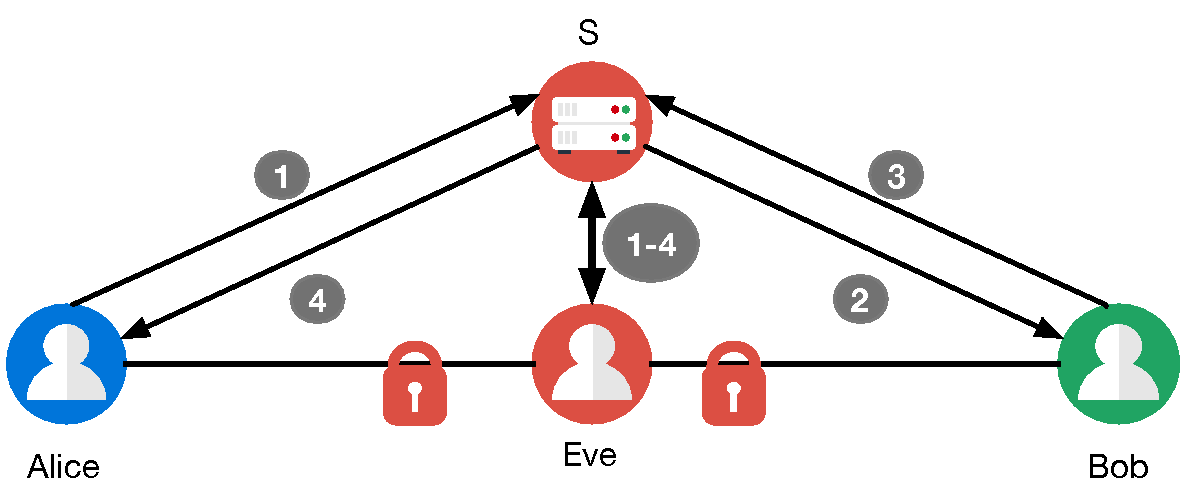
\includegraphics[width=.8\textwidth]{images/mitm}
\caption[WebRTC Man-in-the-Middle Attack]{WebRTC Man-in-the-Middle attack. The \gls{sdp} messages are: (1) Alice's offer relayed to Eve, (2) Eve's offer impersonating Alice, (3) Bob's anwser, (4) Eve's answer.}
\label{fig:mitm}
\end{figure}

To solve this issue, WebRTC proposes a mechanism for peers to authenticate to one another using an \gls{idp} as a trusted third party.
We refer to this mechanism as the WebRTC identity architecture, presented in Figure~\ref{fig:webrtcDeployId}.
To authenticate, peers bind their session fingerprint to a human readable identity by providing an identity assertion.
This identity assertion covers two main claims: the user identifier and the session fingerprint used.
By verifying the assertion and comparing it to the received session fingerprint attribute, peers can authenticate the other peer and verify that no man-in-the-middle attack is being mounted.

\begin{figure*}
\centering
\begin{subfigure}{\textwidth}
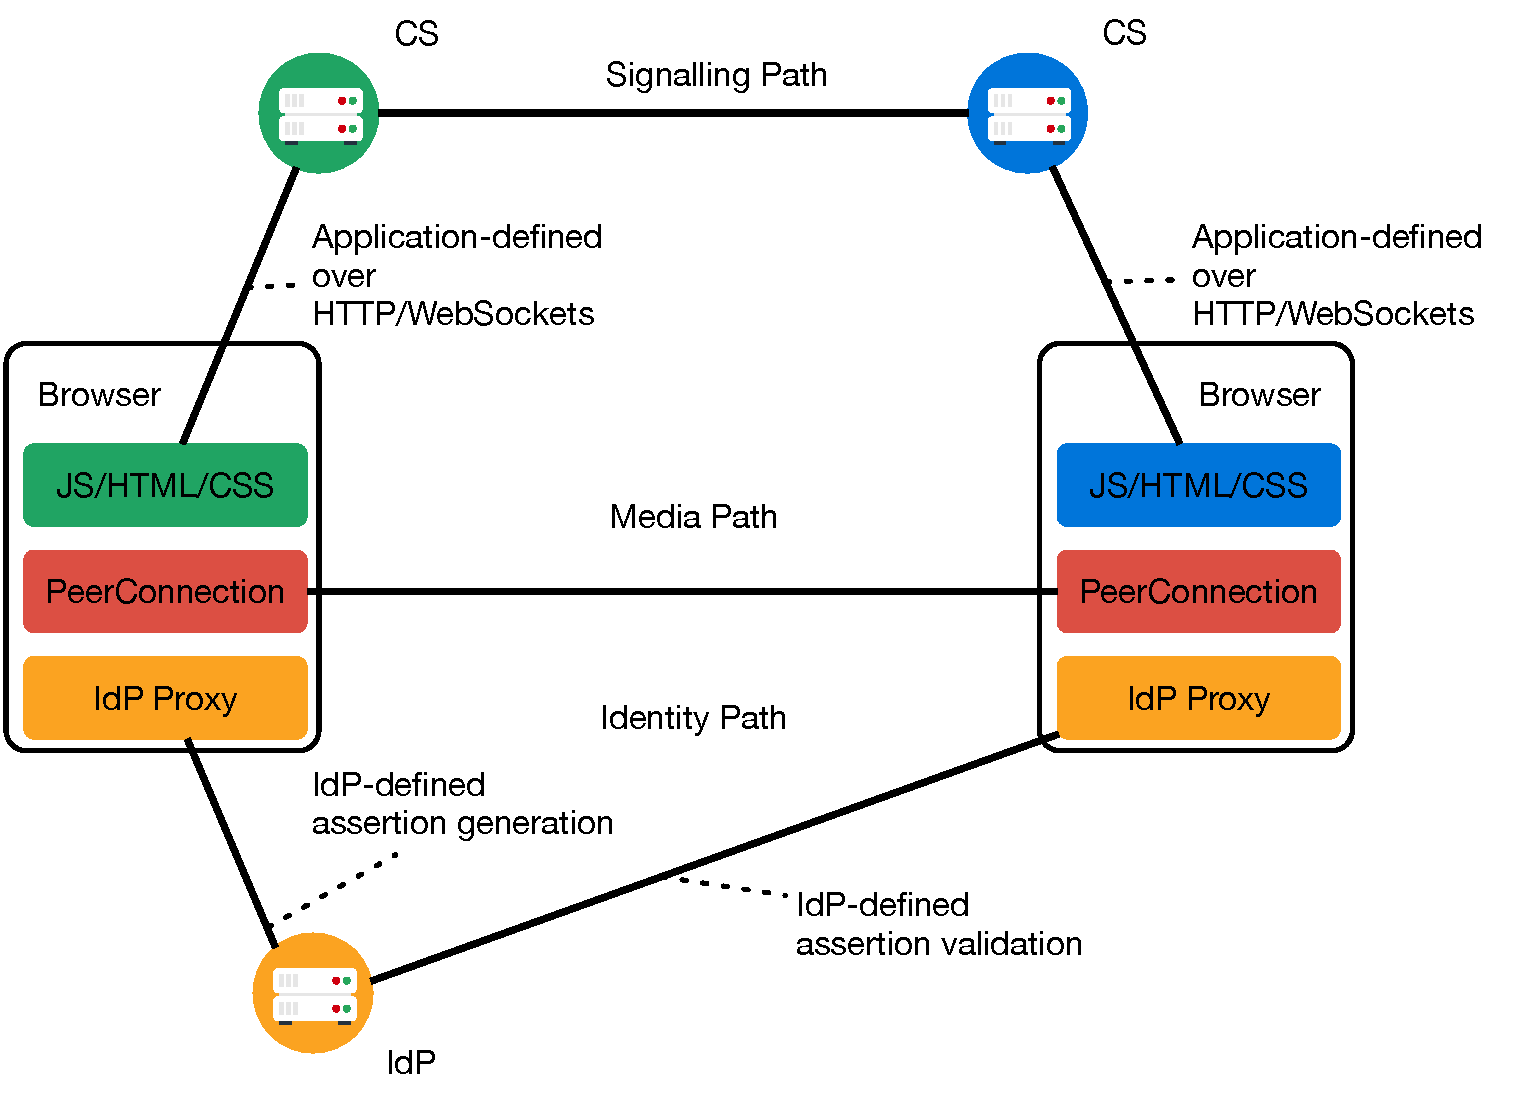
\includegraphics[width=.9\textwidth]{images/webrtcDeploymentId}
\caption[WebRTC deployment with two browser endpoints]{WebRTC deployment with two browser endpoints, two signalling servers, and a single identity provider authenticating the left-side peer.}
\label{fig:webrtcDeployId}
\end{subfigure}
~
\begin{subfigure}{\marginparwidth}
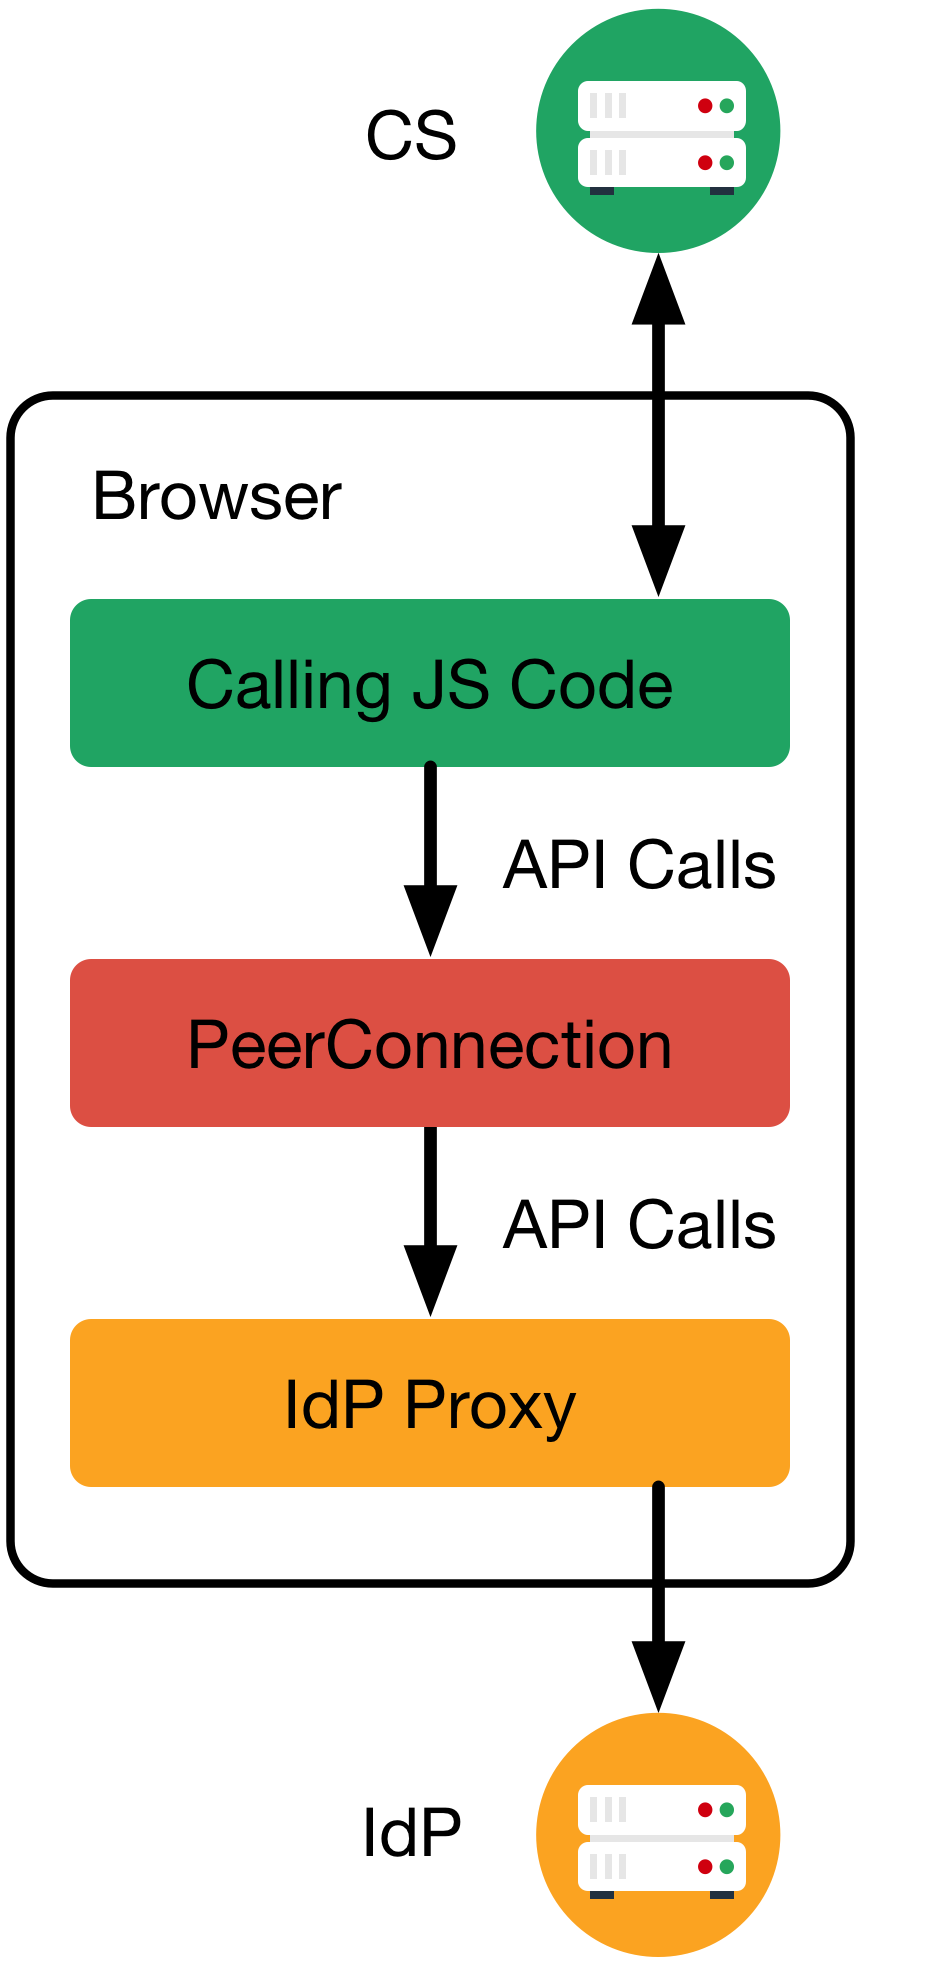
\includegraphics[width=\marginparwidth]{images/webrtcIdPProxyArch}
\caption{WebRTC Identity API Architecture}
\label{fig:webrtarch}
\end{subfigure}
\caption{WebRTC Identity Architecture}
\end{figure*}

In order to enable the generation and the verification of identity assertions from any authentication delegation protocol and providers, the WebRTC security architecture~\cite{I-D.ietf-rtcweb-security-arch} specifies the \gls{idp} Proxy component.
This component serves as an interface between the WebRTC PeerConnection object and the \gls{idp} through the interface presented in Figure~\ref{idProxyWebIDL}.
The \gls{idp} Proxy is available at a well-known location on the \gls{idp} domain.
Before making an \gls{sdp} call offer or answer, the PeerConnection calls the \gls{idp} Proxy to generate an assertion covering the session fingerprint.
After the \gls{idp} authenticated the user, the identity assertion is returned.
This assertion is then included in the \gls{sdp} message in an \texttt{a=identity} attribute, along with the \gls{idp} Proxy location on the \gls{idp} domain.
This allows peers to discover \gls{idp} Proxy location without prior knowledge or relationship with the \gls{idp}.
On receiving an \gls{sdp} message containing an Identity Assertion, the PeerConnection object downloads the \gls{idp} Proxy from the specified location.
It then calls the \gls{idp} Proxy's assertion verification function.
If the verification is successful, the session fingerprint and the user identity are returned.

\begin{figure}[H]
\begin{Verbatim}[commandchars=\\\{\}]
dictionary \textcolor{matred}{RTCIdentityProvider} \{
    \textcolor{matred}{generateAssertion}(
        \textcolor{matblue}{DOMString}                    contents,
        \textcolor{matblue}{DOMString}                    origin,
        \textcolor{matred}{RTCIdentityProviderOptions}   options,
    ),
    \textcolor{matred}{validateAssertion}(
        \textcolor{matblue}{DOMString}                    assertion,
        \textcolor{matblue}{DOMString}                    origin,
    )
\end{Verbatim}
\caption{Interface Exposed by Identity Providers in WebIDL.}
\label{idProxyWebIDL}
\end{figure}

The WebRTC specification allows users to choose a default \gls{idp} in their browser preferences if none was specified by the \gls{cs}.
But implicitly, if the \gls{cs} sets up an \gls{idp} to authenticate a WebRTC call, we would expect it to be the same \gls{idp} used to sign into the \gls{cs}'s website.
Indeed, the \gls{cs} must be able to handle the authentication procedure and needs to know that the user has an active account on this \gls{idp}. 
Besides, from a user experience perspective, it is important that the identity presented on the \gls{cs} webpage and the one received in the identity assertion are consistent with each other.
In practice, the choice of \gls{idp} would thus be defined by the \gls{cs} and limited in the same way as for common authentication delegation services.
We refer to this constraint as \textit{identity continuity}.


\subsection{Considered Protocols for WebRTC Peer Authentication}
\label{sec:authProtocol}
In this section, we present the authentication delegation protocols considered for integration with the WebRTC identity architecture~\cite{I-D.ietf-rtcweb-security-arch}.
These protocols are the BrowserID - Mozilla Persona protocol and the OAuth~2 protocol and its identity extension OIDC.
Figure~\ref{idmstandards} replace these protocols in the history of standards and technologies for user identity management.
As it is a technical prerequisite to both protocols, we first explain the JSON Web Token standard.  

\begin{figure*}
\centering
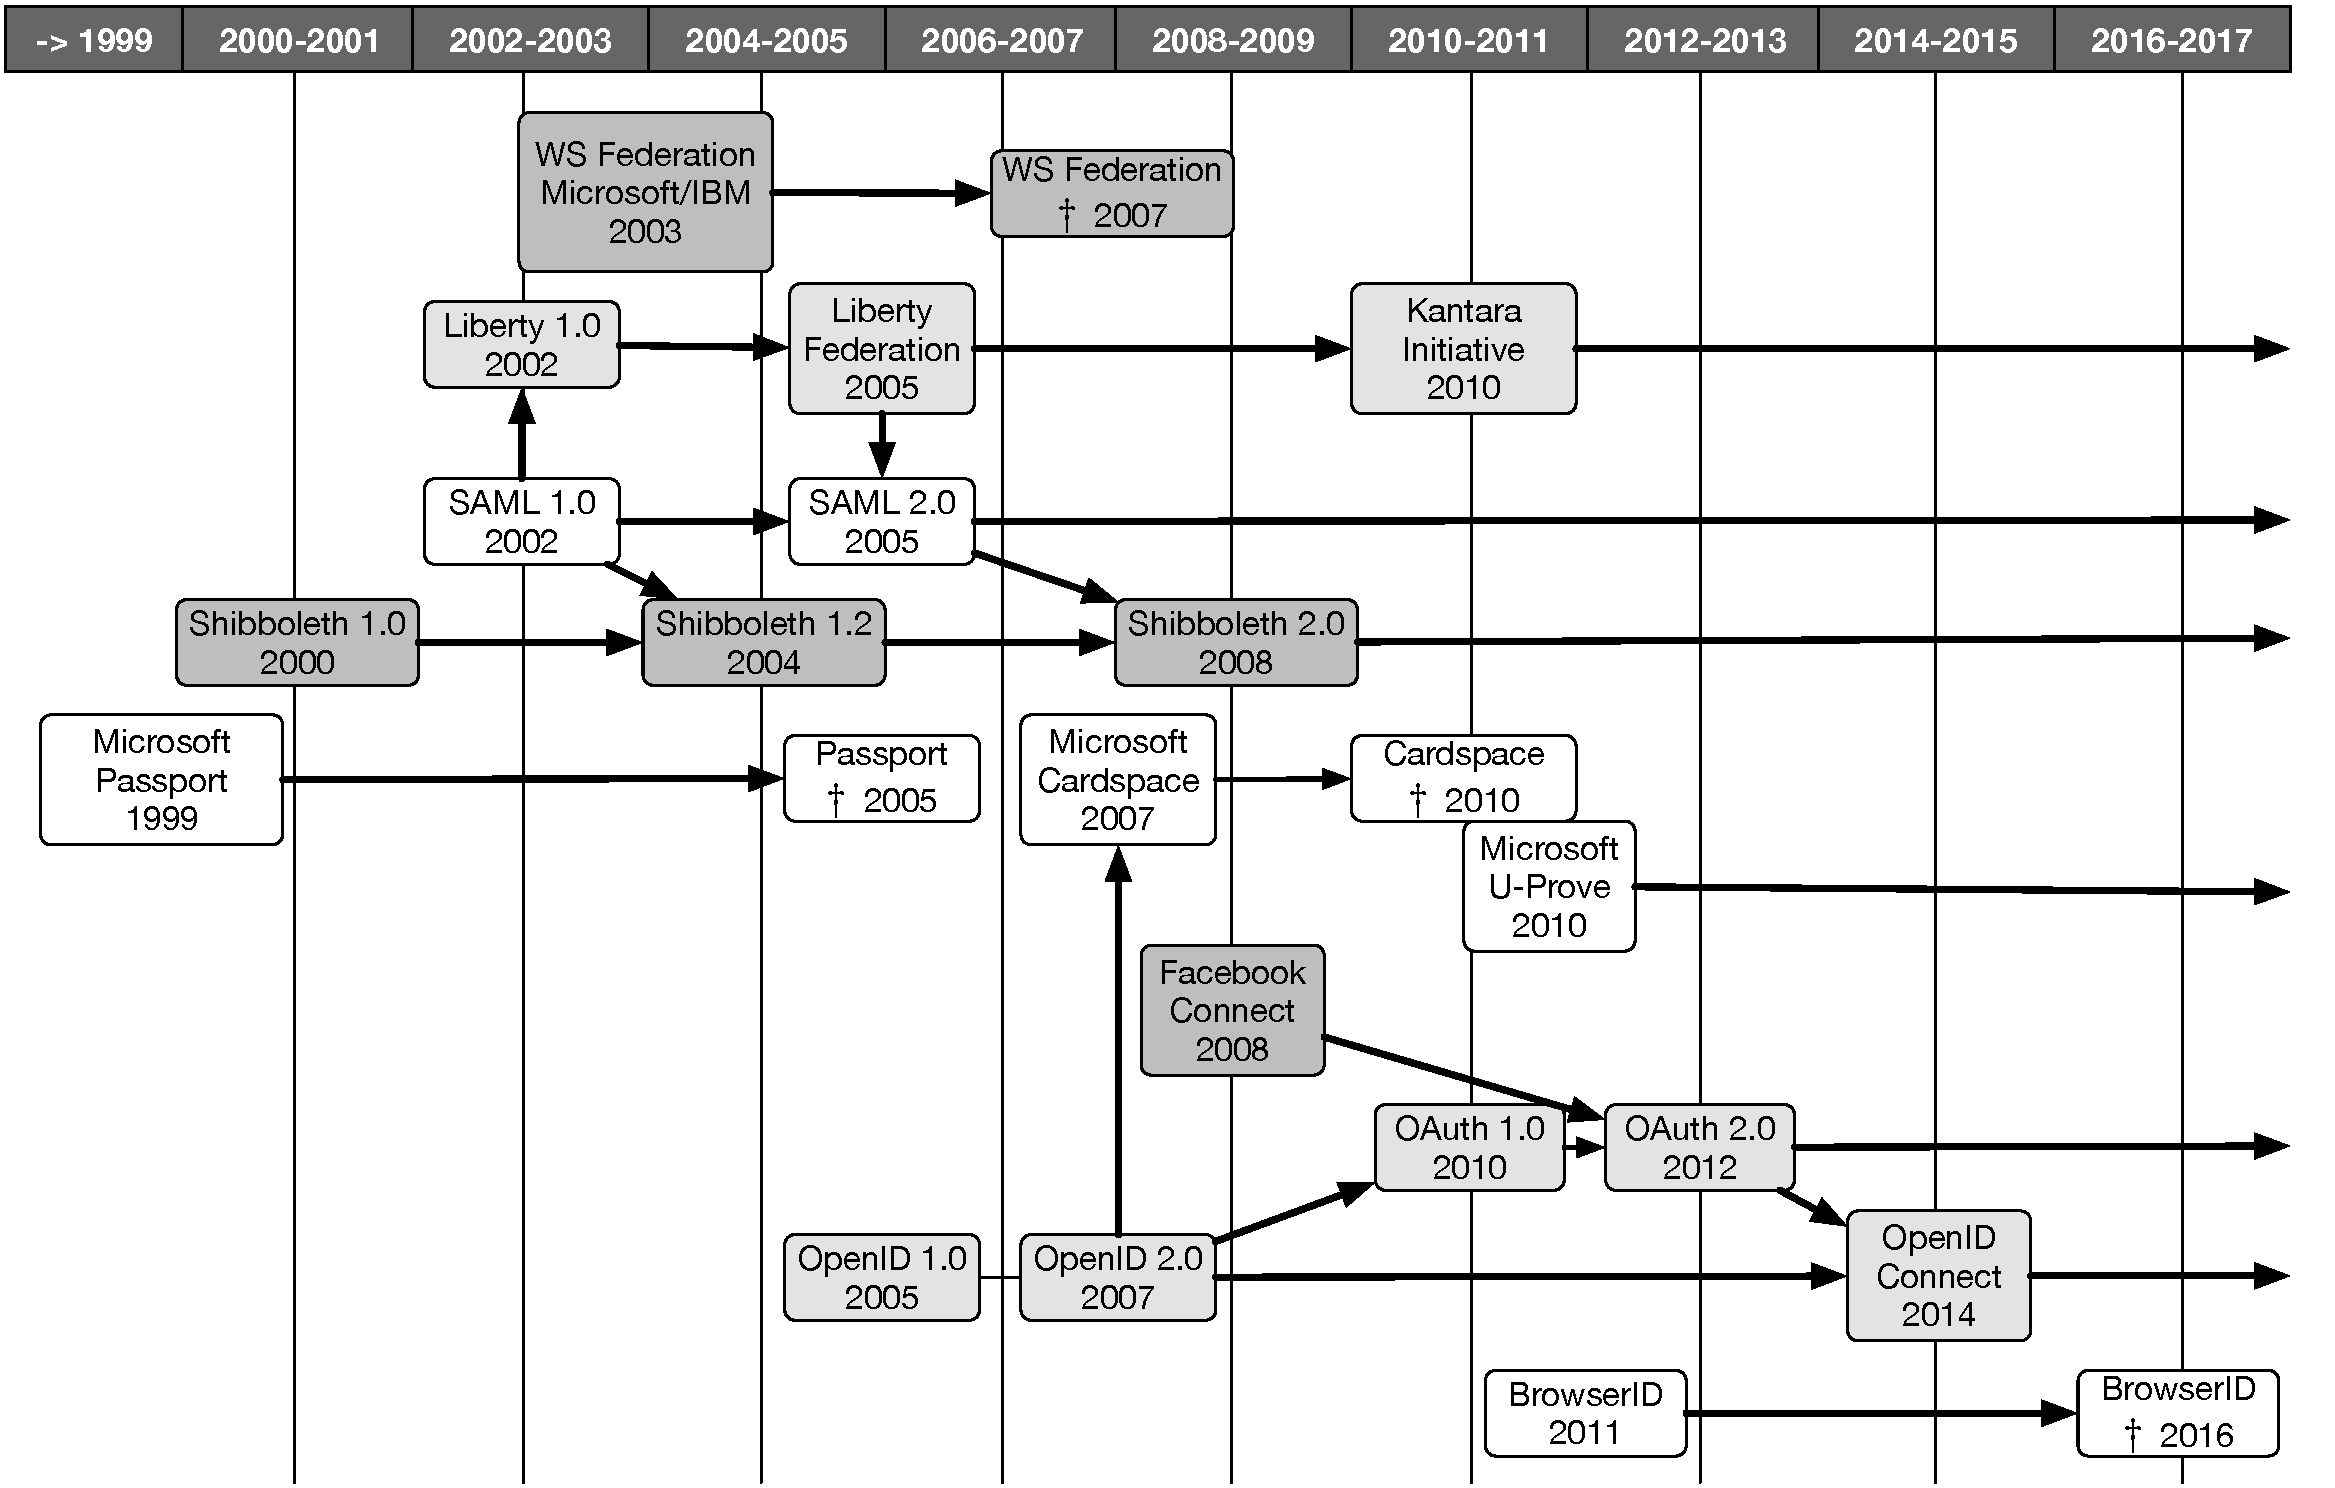
\includegraphics[width=\overflowingheadlen]{images/idmstandards}
\caption{Evolution of standards and technologies for user identity management, updated from J{\o}sang's 2014 survey~\cite{josang14}.}
\label{idmstandards}
\end{figure*}

\subsubsection{JSON Web Token}
\label{jwt}
\gls{jwt}, specified by \gls{rfc}~7519~\cite{RFC7519}, is a way of representing claims to be exchanged by two parties.
These claims are encoded in a \gls{json}~\cite{RFC7159} object which can then be signed as a \gls{jws}~\cite{RFC7515} or encrypted as a \gls{jwe},~\cite{RFC7516}.
\gls{jws} and \gls{jwe} tokens contain several \gls{json} members and in particular, a header and a payload or cyphertext, \ie the \gls{jwt} claims set.
These tokens can be compactly serialised by concatenating their base~64 encoded members.
The acronym \gls{jwt} is commonly used in place of \gls{jws} or \gls{jwe} depending on the context.

For instance, the following set of claims describes the subject \texttt{248289761001} whose name is \texttt{Jane Doe}.
The token was issued by \texttt{http://server.example.com} at \texttt{1509105796} seconds since the \gls{posix} Epoch, \ie January the 1st of 1970.

\begin{verbatim}
{
  "iss": "http://server.example.com",
  "sub": "248289761001",
  "aud": "s6BhdRkqt3",
  "nonce": "n-0S6_WzA2Mj",
  "exp": 1509192196,
  "iat": 1509105796,
  "name": "Jane Doe",
  "given_name": "Jane",
  "family_name": "Doe",
  "gender": "female",
  "birthdate": "1987-01-01",
  "email": "janedoe@example.com",
  "picture": "http://example.com/janedoe/me.jpg"
}
\end{verbatim}

The following \gls{jose} header describes the usage of the \texttt{RS256} algorithm and the key with id \texttt{1e9gdk7}.
RS256 is the compact representation of the \texttt{RSASSA-PKCS-v1\_5 using SHA-256} algorithm, \ie a public key signature algorithm.

\begin{verbatim}
{"kid":"1e9gdk7","alg":"RS256"}
\end{verbatim}

Serialisation of this token is done by encoding both components in base~64 and concatenating them separated by a dot.
The signature is then computed by using this string and the specified algorithm and appended to the serialised token.
The following text is the previous \gls{jwt} and \gls{jose} header examples signed into a \gls{jws}. 
The red part is the header, the violet is the \gls{jwt} payload, and in blue is the signature~\footnote{}.

\begin{figure}[H]
\begin{Verbatim}[commandchars=\\\{\}]
    \textcolor{matred}{eyJraWQiOiIxZTlnZGs3IiwiYWxnIjoiUlMyNTYifQ}.\textcolor{matviolet}{eyJpc3MiOiJodHRwOi}
    \textcolor{matviolet}{8vc2VydmVyLmV4YW1wbGUuY29tIiwic3ViIjoiMjQ4Mjg5NzYxMDAxIiwiYXV}
    \textcolor{matviolet}{kIjoiczZCaGRSa3F0MyIsIm5vbmNlIjoibi0wUzZfV3pBMk1qIiwiZXhwIjox}
    \textcolor{matviolet}{NTA5MTkyMTk2LCJpYXQiOjE1MDkxMDU3OTYsIm5hbWUiOiJKYW5lIERvZSIsI}
    \textcolor{matviolet}{mdpdmVuX25hbWUiOiJKYW5lIiwiZmFtaWx5X25hbWUiOiJEb2UiLCJnZW5kZX}
    \textcolor{matviolet}{IiOiJmZW1hbGUiLCJiaXJ0aGRhdGUiOiIxOTg3LTAxLTAxIiwiZW1haWwiOiJ}
    \textcolor{matviolet}{qYW5lZG9lQGV4YW1wbGUuY29tIiwicGljdHVyZSI6Imh0dHA6Ly9leGFtcGxl}
    \textcolor{matviolet}{LmNvbS9qYW5lZG9lL21lLmpwZyJ9}.\textcolor{matblue}{iYiil5mBuznlG5aGMnOeHkVALg41q1aK}
    \textcolor{matblue}{BFCoXW2f5sth3mZtkCwaRWUbj18pMN7iXlJOOdp9YVthccXORflV1hHlMKnrI}
    \textcolor{matblue}{aqlsoTo6aSnAHVgCJc64pKKMTOsIF0EVhcJ-obigxx0UOvme8AV1oQQkn8Bzc}
    \textcolor{matblue}{2Dd9E5D0qJX5YbeDw}
\end{Verbatim}
\caption[A JWT Example: OIDC ID~Token]{A JWT Example: OIDC ID~Token. Visit \url{https://jwt.io} to decode the token. It can also be verified using the following public key: 

\footnotesize{\texttt{-{}-{}-{}-{}-BEGIN PUBLIC KEY-{}-{}-{}-{}-
MIGfMA0GCSqGSIb3DQEBAQUAA4
GNADCBiQKBgQCrpVE2fAdanHGf
HA10RkmNPIFvCry5XMccRguIGR
zU9wgVBfJ+UeChN9GmcmGf67bE
GbtOY7mScWidKpm3u+XZUOXfl3
PQTF3kIPzKU2cOUwDeziHRmGKR
QXvtTy2esBH45GKzKjFHH6ti6o
Uy3QG7wSZ7kXGGS6pgXjkPBU6y
qwIDAQAB\\
-{}-{}-{}-{}-END PUBLIC KEY-{}-{}-{}-{}-}}}
\label{fig:jwt}
\end{figure}

\subsubsection{BrowserID - Mozilla Personna}
\label{sec:browserid}
BrowserID~\cite{browserid-specs} was Mozilla's attempt at a decentralized \gls{sso} protocol. 
Though it has been deprecated in 2016 due to a declining usage, the protocol was a central example of the WebRTC identity architecture~\cite{I-D.ietf-rtcweb-security-arch} interoperability claim.
Mozilla Persona was the BrowserID service hosted by Mozilla and using a simple email ownership verification mechanism to authenticate users.
The reason for the failure of BrowserID is probably that it did not attract enough interest from potential \gls{idp}.

BrowserID adds the \textit{id} property to the browser's \textit{window.navigator} object.
This property exposes several functions allowing a website client script to request an identity assertion from the browser.
The browser responds to identity assertion requests with a signed \gls{jwt}.
This \gls{jwt} contains the user identifier and a certificate for the user's public key corresponding to the \gls{jwt}'s signature.
The \gls{idp}'s public key verifying the certificate is publicly exposed on the \gls{idp}. 
Any website can verify the certificate's signature thus establishing a trust chain from the user to the \gls{idp}.

The BrowserID protocol allows any domain to be used as an \gls{idp} by signing a certificate for the user.
The user identifier must be an email address whose domain corresponds to the \gls{idp}'s domain name.
The email's domain allows \gls{idp} discovery as the location of the \gls{idp}'s public key and other endpoints are standardised on a \texttt{/.well-known} route.
The browser stores user's certificates and is then responsible for signing identity assertion for requesting website.
This separation of functionalities between the \gls{idp} and the browser allows for a privacy-friendly approach as the \gls{idp} is not aware of which site is the user login into.

Hiding the user's login actions behind a trusted component is also an approach proposed by Orange with the Trusted Identity Module~\cite{tim}.
Similarly, our technique described in the patent for a Method of managing the authentication of a client in a computing system~\cite{corre_authent} protects user privacy by putting the identity assertion in a decentralised network such as a blockchain.
In these architectures, the \gls{idp} cannot monitor who is verifying the identity assertion.


\subsubsection{OAuth 2 and OIDC}
\label{sec:oauth2}
\label{sec:oidc}

\begin{figure}
\begin{subfigure}{.3\textwidth}
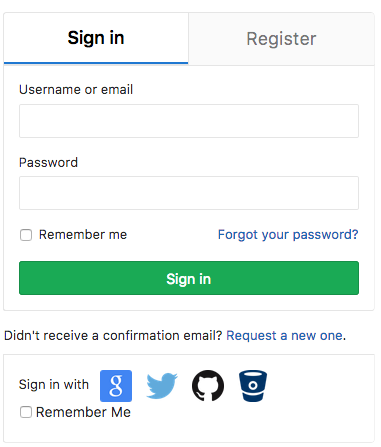
\includegraphics[width=\marginparwidth]{images/signinGitlab}
\caption[Sign in page]{GitLab sign in page with a selection of IdP.}
\label{fig:signinGitlab}
\end{subfigure}
~
\begin{subfigure}{.3\textwidth}
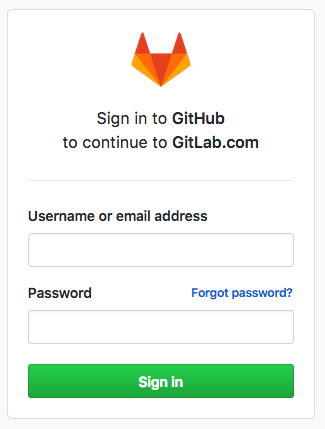
\includegraphics[width=\marginparwidth]{images/authnGitlab}
\caption[Redirection page]{Redirection to Github sign in page for Gitlab.}
\label{fig:authnGitlab}
\end{subfigure}
~
\begin{subfigure}{.3\textwidth}
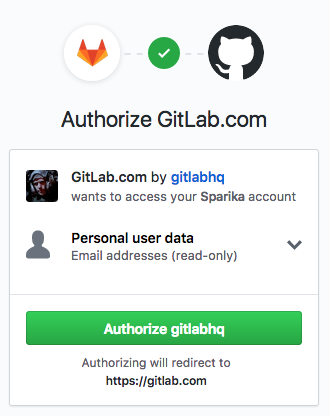
\includegraphics[width=\marginparwidth]{images/authzGitlab}
\caption[Consent page]{Github consent page to share email with Github.}
\label{fig:authzGitlab}
\end{subfigure}

\caption[OAuth~2 Process Example]{OAuth~2 process involving Github as AS and RS, and Gitlab as client.}
\label{fig:oauth2Gitlab}
\end{figure}

With more and more content being published by users, websites and in particular social networks need a way to securely expose their \gls{api}.
In order to respect users' privacy, it is, however, necessary to get users' consent to share private information. 
The original OAuth specification was published in 2006 as a solution to the problem of authorization delegation.
OAuth was then standardised by RFC~5849~\cite{RFC5849} and later deprecated by RFC~6749~\cite{RFC6749}: the OAuth~2.0 protocol.

The OAuth~2 specification defines four roles.
The \gls{ro}, in most case a user, is legally capable of granting access to the resource.
The \gls{rs} is where the resource is hosted.
The Client is the application requiring access to the resource on behalf of the resource owner and with its authorization.
Finally, the \gls{as} can grant an access token to the client after getting the resource owner consent.

The main OAuth~2 protocol flow is called the code flow, represented in Figure~\ref{fig:oauthsequence}.
Figure~\ref{fig:oauth2Gitlab} shows the user actions in such a flow.
An OAuth~2 flow is based on \gls{http} and make use of redirection response (code 300) to let servers exchange information on behalf of the user.
In this flow, the client makes an \gls{http} request for an authorization from the \gls{ro} for a specific resource (1 in Figure~\ref{fig:oauthsequence}).
The \gls{as} authenticates the user (Figure~\ref{fig:authnGitlab}) and then asks for his consent (Figure~\ref{fig:authzGitlab}).
The requested authorizations are transmitted to the \gls{as} in the \textit{scope} parameter of the \gls{http} authorization request.
After the \gls{as} got the user's consent, the request is redirected to the client (2).
This redirection contains an authorization code, for instance in the URL query parameter, which can be retrieved by the client.
The client then exchanges the authorization code with the \gls{as} for an access token (3, 4).
This exchange happens out of the \gls{ro} scope and allows the \gls{as} to authenticate the client.
The access token is then used to access the resource on the \gls{rs} (5,6).
In order to be authenticated by the \gls{as}, the client must be registered.
The process of registration most often involves the client's developer taking manual actions to register on the \gls{as} through HTML forms.
However, automatic discovery and registration are also possible if the \gls{as} exposes some metadata and registration endpoints.
%Although specifications for automatic discovery and registration exist for both OAuth~2 and OpenID Connect, we show in \ref{OAuth study} that they are not implemented by AS.

\begin{figure}
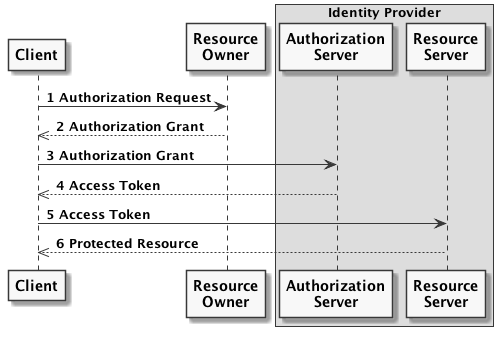
\includegraphics[width=.78\textwidth]{images/oauth2}
\caption{Abstract Oauth~2 code flow taken from RFC~6749.}
\label{fig:oauthsequence}
\end{figure}

In the alternative implicit flow, the \gls{as} directly responds to the authorization request with the access token rather than with an authorization code. 
This simplified flow is adapted for client implemented in the browser rather than on a server.
In such scenario, the client code is visible from the user and cannot protect a secret key. 
As a result, the client cannot be authenticated by the \gls{as} and the authenticated authorization grant is unnecessary.
However, the resulting process is less secure as the access token may be exposed on the web browser.

While OAuth~2 is able to convey user authentication information, it does so in non-standard ways left for implementors to decide.
Actually, authentication in OAuth~2 is implicit as it is assumed that the user was authenticated by the \gls{as} in order to get the user's consent.
For the client, getting the user's email means that the owner of the email has been authenticated, but it does not know much more than that.

\glsreset{oidc}
\gls{oidc}, developed by the OpenID foundation, is ``a simple identity layer on top of the OAuth 2.0 protocol''~\cite{sakimura_openid_2014}.
It allows clients to retrieves an ID~Token in parallel from the access token.
This ID~Token is a \gls{jwt}, containing information related to the user's identity, as the one in Figure~\ref{fig:jwt}.
In addition to the ID~Token and additions to the OAuth~2 protocol, OIDC standardises a set of identity claims.
A client using OpenID Connect and requesting an ID~Token must add the \textit{openid} scope to his OAuth~2 authorization request.
The received ID~Token contains a list of attributes describing the user's authentication result.
In particular, the triple of identifiers \textit{iss}, \textit{sub}, \textit{aud} respectively identify the token ISSuer (\ie the \gls{as}), the SUBject (\ie the user), and the token AUDience (\ie the client).
The audience identifier certifies to the client that it is the intended audience of the token and is not subject to replay attacks.
Note that to avoid correlation attacks (as described in Section~\ref{sec:privacy}), the subject identifier must be locally unique \ie the same user must not have the same \texttt{sub} identifier for two different clients.
The ID~Token also contains expiration time and security parameters such as authentication time, nonce, and authentication level.
The requested claims describing the user identity can either be contained in the ID~Token or retrieved from the UserInfo endpoint.
This endpoint is an OAuth~2 protected resource that can be accessed with a valid access token for the \texttt{openid} scope.
While \gls{oidc} standardises a set of identity claims, additional claims can be added freely to both the ID~Token and the UserInfo endpoint as long as they use collision-resistant names or that naming conflicts are unlikely.

From a user's point of view, the difference between OAuth~2 and \gls{oidc} flows should not be visible.

\subsection{Alternative Key Management Protocols}
\label{sec:keymanagement}
\gls{dtlssrtp} and \gls{dtls} in conjunction with the use of the identity path allow to bind negotiated keys to an identity authenticated by an \gls{idp}.
Although these are the default and preferred key management protocols respectively for media and data channels, alternative key management protocols offer different security guarantees.
In this section, we present the SDES and ZRTP protocols.

The \gls{sdes}~\cite{RFC4568} was the main competitor to \gls{dtlssrtp} as the default security protocol for WebRTC.
The main advantage of \gls{sdes} consists in its existing deployment in existing \gls{sip}/\gls{rtp}~\cite{I-D.ohlsson-rtcweb-sdes-support} based \gls{voip} networks\footnote{VoIP designates the techniques to communicate using voice or voice and video over any compatible \gls{ip} networks.}.
In particular, interconnectivity between WebRTC and \gls{sip}/\gls{rtp} endpoints would require the deployment of media gateways.
As media gateways are complex and costly to implement, leveraging the existing implementations of \gls{sdes} gateways would reduce costs and favour WebRTC interconnectivity.
Additionally, due to the existing \gls{sdes} deployment, gateways may not have to decrypt/encrypt session negotiated with \gls{sdes} thus achieving end-to-end encryption.
However, contrary to \gls{dtls}, in the \gls{sdes} protocol keys are exchanged in clear over the signalling path inside \gls{sdp} messages.
This implies that the \gls{cs} can decrypt the streams invisibly.
While this seems to be a major vulnerability, in the context of real-time communication it may be a legit requirement from \gls{cs} as they may be subject to lawful interception requirements.
In comparison, mounting lawful intercept against \gls{dtlssrtp} is mainly possible through a \gls{mitm} interception as described earlier\footnote{Note that in interconnectivity scenarios, gateways can decrypt \gls{dtlssrtp} streams unless both endpoints are using \gls{dtlssrtp} in conjunction with verified identity assertions.}.
\gls{dtls} was considered by the \gls{ietf} as offering stronger security guarantees and qualified as mandatory to implement.
Furthermore the implementation of both the \gls{dtls} and \gls{sdes} protocols may allow for a downgrade attack.
To implement such attack, a malicious service would have to modify the \gls{sdp} messages to only advertise \gls{sdes} support.
As a result, peers could negotiate a lower security level, allowing the service to then mounts an invisible interception attack. 
Not only was \gls{dtlssrtp} preferred over \gls{sdes}, but \gls{sdes} was also not authorized for implementation in WebRTC endpoints.

\marginpar{
\captionsetup{type=figure}
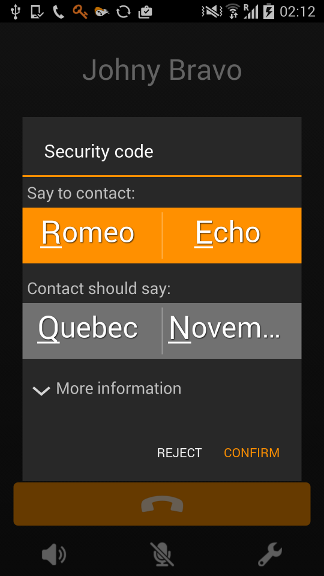
\includegraphics[width=\marginparwidth]{images/zrtp}
\caption{Phone-X application displaying the ZRTP SAS.}
\label{fig:zrtp}
}

The ZRTP protocol~\cite{RFC6189} is a media path keying protocol for \gls{srtp}.
It uses a simple Diffie-Hellman exchange to agree on the symmetric session key.
A \gls{sas} is then derived from the session-key and vocally transmitted over the media path (see Figure~\ref{fig:zrtp}).
As both peers compare the exchanged \gls{sas}, \ie $hash(K_A) = hash(K_B)$, they get a confirmation that they negotiated the same session-key and that no MitM is being set up, \ie $K_A = K_B$. 
Although the \gls{sas} comparison is vulnerable to a real-time audio spoofing attack, in practice it is quite complicated.
Indeed, to succeed and remain undetected, the attacker must inject his own \gls{sas} at the right moment.
This requires detecting, how, when, and which one of the peers will say the \gls{sas}.
Video session may further deter such attack.
However, practical attacks and bugs on ZRTP implementations have been recently reported~\cite{SchurmannKHW17}.
As a matter of fact, ZRTP is currently implemented by multiple \gls{voip} clients offering end-to-end encryption.
But their reliance on the \gls{sas} vocal comparison procedure and their implementations of different security indicators and procedures may be confusing for most users.
ZRTP is also less flexible than the \gls{idp} Proxy solutions of WebRTC as it is only adapted for the \gls{voip} use case.
WebRTC data channels, uni-directional communications, or non-human peer use cases cannot be secured by ZRTP.









%%%%%%%%%%%%%%%%%%%%%%%%%%%%%%%%%%%%%%%%%%%%%%%%%%%%%%
%%%%%%        TRUST
%%%%%%%%%%%%%%%%%%%%%%%%%%%%%%%%%%%%%%%%%%%%%%%%%%%%%%

\section{Trust}
\label{sec:trustintro}
Evaluating the security of a system is only possible if it can be observed and monitored.
In communication scenarios, only a fragment of the whole system is under the user control.
The rest of the system is controlled by other peers, certificate authorities, communication service providers, identity providers, and public internet service providers or enterprise network administrators.
If a complete monitoring is not possible, it may be necessary to make a trust decision.
In this section, we define trust and the properties often associated with formal trust models.
We then explain the actual WebRTC trust model.

\subsection{Introduction on Trust}
Experienced every day, trust is nonetheless hard to define due to the broad range of situations and interactions it covers. 
Several definitions of trust have been proposed.
Inspired by McKnight and Chervany~\cite{mcknight1996meanings}, J{\o}sang and Presti define trust as: ``\textbf{the extent to which one party is willing to depend on something or somebody in a given situation with a feeling of relative security, even though negative consequences are possible}''~\cite{josang2004analysing}.
In the sense of an action, we would say that trust is the decision of intelligent agents to cooperate in the face of risk and uncertainty about the behaviour (capability or intention) of other agents.
This heuristic is often based on prior interaction history, reputation from a community, or recommendations from other trusted sources.

A truster is a person, an organisation, or a software agent while a trustee is an agent, possibly non-intelligent, that can provide a service to the truster.
Figure \ref{fig_trust} presents such a simple trust relationship.
Trust between two agents is asymmetric and depends on a specific context, \ie a specific scope of action for which trust is granted. 
Transitivity is a property commonly associated with trust relationship where an agent D would recommend its trust in E to B (see Figure~\ref{fig_trustnet}).
As capability in a given context does not imply the capability to recommend other agents in the same field of expertise, transitivity is not present in all models.
However, a recommendation could be seen as a context allowing transitivity to other contexts.
Indeed, J{\o}sang and Pope describe a transitive path as a chain of recommending trust terminated by a functional trust~\cite{josang2005semantic}. 
Trust recommendation can also be aggregated from multiple sources.
Figure~\ref{fig_trustnet} shows trust transitivity and aggregation. 
Dashed arrows represent recommendations, while the dotted arrow represents the trust relation from A to E built from recommendations aggregation. 


\marginpar{
\centering

\captionsetup{type=figure}
\caption{Trust representation}
\label{fig_trust2}

\captionsetup{type=subfigure}
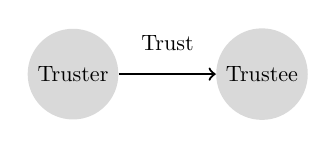
\begin{tikzpicture}[transform shape, scale=.8]
\node(A)[circle, fill=gray!30] at (0,0) {Truster};
\node(B)[circle, fill=gray!30] at  +(3,0) {Trustee};
\node(T) at  +(1.5,0.5) {Trust};
\draw [->][thick] (A) -- (B);
\end{tikzpicture}
\caption{Trust relationship}
\label{fig_trust}
\bigskip

\captionsetup{type=subfigure}
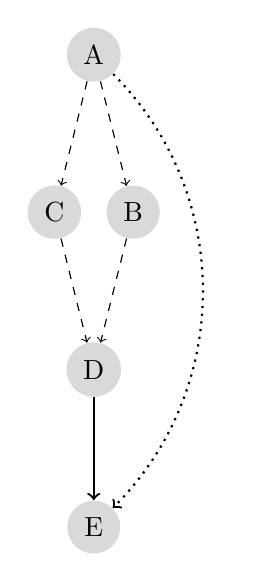
\begin{tikzpicture}[transform shape]
\tikzstyle{every node} = [circle, fill=gray!30]
\node(A) at (0,6) {A};
\node(B) at  +(.5,4) {B};
\node(C) at  +(-.5,4) {C};
\node(D) at  +(0,2) {D};
\node(E) at  +(0,0) {E};
\foreach \from/\to in {D/E}
\draw [->][thick] (\from) -- (\to);
\foreach \from/\to in {A/B, A/C, B/D, C/D}
\draw [->][dashed] (\from) -- (\to);

\draw [->][dotted, thick] (A) to [out=-45,in=45] (E);

\end{tikzpicture}
\caption{Trust transitivity}
\label{fig_trustnet}
\medskip

}

Methods to establish trust are commonly categorised between policies and reputation based~\cite{artz2007survey}:
\begin{itemize}
\item Policies describe the ``hard evidence'' requirements to obtain trust in a situation where trust in an agent itself is unknown but there is an existing trust in a third party authority. 
\item The concept of reputation describes the perception of a community on the reliability of an agent part of this community for a particular context.
%An opinion is a subjective view of an agent about another agent's past behaviour. 
%Reputation in a community is thus formed by the aggregation of opinions by means of recommendation. 
These recommender systems are either organised by a trusted third party or in a peer-to-peer fashion.
Furthermore, recommender systems can only establish a reputation in a network where data about agents' behaviour is available.
\end{itemize}

Trust relationships are dynamic as new feedback and credentials creation or revocation will impact previously existing trust. In some models, recommendations are part of this dynamic as delay can occur in a trust information propagation.
Time may also play an important role in trust dynamic, either as an ageing factor determining ponderation of new experience over previous ones or as an eroding factor decreasing trust or the precision of a trust value. 

Various trust metrics have been proposed ranging from discrete or fuzzy to continuous scale~\cite{artz2007survey}.
We observe two categories of trust measure representations that differ from their representation of distrust. 
The first category represents trust on a scale of $[-x;+x]$ with the negative value representing distrust, and zero a neutral trust.
The second category uses a scale of $[0;x]$ with 0 representing full distrust.
In the first case, a bad recommendation by a distrusted source contributes positively to the final trust level, while on the second computational model, the recommendation would simply be discarded due to a low ponderation.
Other representations can be considered as a special case of these two categories.

Authors in the literature~\cite{mui2002computational,josang2006exploring} define operators for trust relationships. In these models, trust transitivity is generally computed with a multiplicative operator while trust sources aggregation is modelled by an averaging operator. Some models may as well represent certainty and distrust. These models handle contradiction in trust recommendation and uncertainty of trust sources. 

\subsection{The WebRTC Trust Model}
From a security perspective, trust is often synonym with ``providing proofs of identity, authorization, and performance''~\cite{artz2007survey}.
Although multiple formal trust models have been proposed and refined in the literature~\cite{artz2007survey}, commercial softwares and services often make use of trust models in a simpler manner.
The current WebRTC trust model is an informal model categorising entities into three categories: the \gls{tcb}, authenticated entities, and unauthenticated entities.

At the root of the model is the WebRTC agent, in most cases a browser, which serves as the \gls{tcb}.
All security properties must be guaranteed by the \gls{tcb}, as we explained in Section~\ref{sec:tcb}.
In particular, the \gls{tcb} is responsible for authenticating other entities acting on the communication.

In WebRTC, authenticated entities are either \gls{cs}, \gls{idp} or other peers.
Optimally, these are cryptographically authenticated by presenting certificates via \gls{https} for servers, and \gls{dtls} or identity assertion for peers.
We previously described in Section~\ref{sec:pubkey} how \gls{ca} build a chain of trust from a root certificate to the final owner's certificate.
The trust chain is then anchored in the browser as it is browser makers who configure the list of root certificates in browsers.
Similarly, the signalling path forms a transitive recommendation path for media session security certificates.
Note that while these entities are authenticated, these may not necessarily be trusted\footnote{``Just because we can verify that https://www.evil.org/ is owned by Dr Evil does not mean that we can trust Dr Evil to access our camera and microphone''~\cite{I-D.ietf-rtcweb-security-arch}.}.
However, it is mandatory to authenticate entities before making a trust decision.
This trust decision is ultimately left for the user to decide.

In particular, while the \gls{cs} has a large control over the WebRTC session, in some scenarios it may be untrusted.
For this reason, the specification introduces an alternative identity path to exchange identity assertions.
These assertions bind media session security certificates to an identity and from a trust perspective, this forms an alternative transitive recommendation path.
Paradoxically, this identity path is left for the \gls{cs} to configure and control as it is the \gls{cs} who sets the \gls{idp} to use.
From our point of view, it is not clear if the identity path can be trusted independently of the \gls{cs}.
%This question underlies RQ3: \textit{Can we let users chose actors they trust to participate in the communication setup?}.

Other network elements are generally not authenticated by the browser.
The WebRTC specification thus assumes that they behave maliciously and the system is supposed to be secure against attacks from these entities.








%%%%%%%%%%%%%%%%%%%%%%%%%%%%%%%%%%%%%%%%%%%%%%%%%%%%%%
%%%%%%        PRIVACY
%%%%%%%%%%%%%%%%%%%%%%%%%%%%%%%%%%%%%%%%%%%%%%%%%%%%%%
\section{Privacy of the Call-Session}
\label{sec:privacy}
Some JavaScript web \gls{api} may expose critical data to malicious websites. 
To protect users these resources must be guarded against unwanted access.
This is done by enforcing explicit consent policies asking users whenever a website requests access to a sensitive \gls{api}.
Permissions may be granted or denied based and websites origin.
\gls{http} origins, considered insecure, are often limited to one time authorizations.
Considerations for privacy in internet standards is steadily increasing\footnote{The battery status \gls{api} was even removed after its implementation in browsers as its benefits were estimated less important than the privacy risk faced by users. This \gls{api} is now only available from privileged code in Firefox~\cite{batteryFF}.}.

\gls{rfc}~4949~\cite{RFC4949} defines privacy as ``the right of an entity (normally a person), acting on its own behalf, to determine the degree to which it will interact with its environment, including the degree to which the entity is willing to share his personal information with others''.
This definition emerged from the United States Privacy Act of 1974. which was concerned with the growing amount of personal data stored by the U.S. government.
In the meantime, the protection of personal data emerged in Sweden, France, and Deutschland, mainly driven by the fear of mass surveillance by an authoritarian state~\cite{usaeuprivacy}.
Privacy should not be used as a synonym for data confidentiality: as a right, privacy is a reason for security rather than a mean.
In this section, we describe types of privacy attack and possible mitigation techniques. 
We also give a brief overview of the legal regulation applying to personal data protection.
Finally, we present existing privacy considerations of the WebRTC security architecture.
%In the rest of the Context part, we will develop privacy consideration when necessary.
%In particular ... \todo{ref to privacy considerations in other context chapter and state of the art.}

\subsection{Attack and Threat Mitigation}
The risks associated with privacy threats are multiple~\cite{RFC6973}.
In the most trivial cases, individuals can suffer from the divulgation of their private life by financial or reputation loss.
Individuals can also feel a sense of unease by knowing or fearing the monitoring of their actions.
This feeling can even lead users to refrain from acting freely.
In the worst case, if the attacker is able to physically harm the individual, the individual's life may be endangered.
\gls{rfc}~6973~\cite{RFC6973} categorise privacy threats between combined security-privacy and privacy specific threats:
\begin{itemize}
\item \textbf{Combined security-privacy threats}
\begin{itemize}
\item Surveillance
\item Stored Data Compromise
\item Intrusion
\item Misattribution or Spoofing
\end{itemize}
\item \textbf{Privacy specific threats}
\begin{itemize}
\item Correlation
\item Identification
\item Secondary Use
\item Disclosure
\item Exclusion
\end{itemize}
\end{itemize}

Particularly related to the context of web real-time communications are the threats of surveillance, misattribution, correlation, and identification.
Surveillance is conducted by an attacker who observes or monitors the individual's communications.
The threat is present even if the communication is encrypted as the possibility of surveillance can lead the individual to change his behaviour, while the fact that the communication is happening may be enough knowledge for the attacker.
Misattribution of behaviour can happen as a result of inadequate or insecure authentication.
Similarly, a privacy attacker may also draw wrong conclusions based on his observations of the individual behaviour. 

Correlation threats are made possible by the combination of pieces of information regarding an individual.
By correlating pieces of information from different sources, an attacker may learn more than what the individual believes to have shared.
Finally, identification is the correlation of an individual's information in order to infer or establish the individual's identity.
For instance, browser fingerprinting techniques can uniquely identify a browser, and its associated user, by executing a set of JavaScript scripts on a website~\cite{laperdrix2016}.
Combined together these technical pieces of information can form a unique and portable identifier, without the user knowledge.

The main solution to mitigate privacy threat is data minimisation.
As it is difficult to define what information can cause a privacy risk, reducing data disclosure globally reduce the privacy attack surface.
Data minimisation is a general principle that should be applied by developers.
The most straightforward approach is to limit data collection to the minimum required, however, a limit may also be set to the time of retention of an information.
In some cases, individuals may themselves enforce data minimisation by reducing the information they expose to websites.
Though this may come as a tradeoff between privacy and functionalities.
If the original value of some data is legitimate, denying its usage can protect an individual's privacy but at a cost.
For instance, most browser fingerprinting techniques rely on the execution of JavaScript.
It is possible to deactivate JavaScript through browser's options but this would break most websites in the process.

An individual is said to be anonymous if it belongs to a set of individuals appearing to have the same attributes.
This set is called an anonymity set and individuals within it must be indistinguishable from each other. 
Anonymity is relative to the point of view of the attacker as it depends on the type of information the attacker can observe.
Additionally, the risk of correlation means that it may be difficult to assess if one belongs to an anonymity set or not.
A slight difference in attributes collected may de-anonymise an individual or at least reduce the size of the anonymity set.
Some privacy preserving approaches thus try to quantify the uniqueness of an attribute.

Respect for privacy recognises the right for an individual to determine to which degree it is willing to interact and share private information with its environment.
For this reason, data collection happening ``in secret'' can be detrimental to an individual's privacy. 
User participation approaches involve the individual in the collection process by asking his consent.
Though modern privacy regulations enforce a strict policy for explicit user consent (see Section~\ref{privacyRegulation}).
Depending on the use case and underlying architecture it may be easier or harder to explicitly ask the user for his consent.

Finally, security in itself is an essential component of privacy protection.
Confidentiality of exchanges and strong peer authentication ensure that data are protected against a malicious third party.

\subsection{Regulations}
\label{privacyRegulation}
Privacy-preserving regulations have been in development since the 1970's both in the USA and in European countries.
Growing concerns by citizens for their privacy on the Internet pushed legislators to adopt more protective legislation.
The new European \gls{gdpr}~\cite{gdpr} is a regulation adopted by the European Parliament in 2016 to reinforce and unify data protection for individuals within the \gls{eu}.

On one hand, the \gls{gdpr} simplify the regulatory environment by unifying it across the \gls{eu}.
On the other hand, the requirements for companies or public entities collecting personal data are more significant.
At the same time, possible sanctions are also more severe going up to 20 000 000 euros or 4\% of the global company revenue.
New principles are also introduced such as privacy by design and by default.
Privacy by design is a concept developed in 1995 by a joint-team from Canada and the Netherlands.
As defined by the \gls{gdpr} in its article 25, privacy by design means that appropriate technical and organisational measures should be taken both at design time and processing time.
The definition of Privacy by default states that appropriate measures should be taken to ensure that only necessary personal data are collected, processed, and stored for each specific purpose of processing.
This principle also comes with an obligation of conformity as soon as the design time of a personal data processing system.
The responsibility to implement and prove conformity regarding the regulation belongs to a Data Protection Officer appointed by each company or public entity.

Major differences oppose the United States and the \gls{eu} regarding how their laws protect the privacy of their citizens~\cite{usaeuprivacy}.
In the United States, privacy is a right recognised by the Constitution in order to protect citizens freedom from the government.
In addition, privacy-preserving laws are decided at the state level rather than at the federal level.
Oppositely, though the \gls{gdpr} also concerns public entities, the regulation is primarily aimed at the \gls{ott} companies often located in the United States. 
For users, the \gls{gdpr} introduces important new rights such as explicit consent, right to be forgotten, right of access, and right of rectification.
Furthermore, the \gls{gdpr} protects \gls{eu} citizens whether the company processing data is located inside or outside the \gls{eu}.
Such protective regulations from the \gls{eu} affect companies across the world forcing them to be compliant.
For these reasons, both United States and \gls{eu} laws are led to interact with each other.
In a similar fashion, several national legislation across the world have been influenced by European laws.

In the meantime, terrorist attacks are pushing governments to adopt new disposition to facilitate the collection and the exchange of data between security services.
While governments reinforce privacy preserving regulations and may invest in privacy-preserving research, communication surveillance is also an ever more important objective for their security services.
As an example of these contradictory efforts, the United States government is both funding research on the Tor network~\cite{DBLP:journals/popets/JohnsonJHSS17} and trying to break it through efforts of the National Security Agency~\cite{ball_nsa_2013}.


\subsection{Privacy Considerations for WebRTC}
The WebRTC security architecture intends to prevent several types of privacy attacks.
Persistent identifiers such as \gls{dtls} certificates allow for correlation attacks against anonymous call.
To prevent this, WebRTC implementations should allow resetting such identifiers, for instance with a similar lifetime as cookies or through a website-controlled mechanism.

\gls{ice} candidates addresses may also form a unique identifier, either by themselves or in conjunction with other web \gls{api} during browser fingerprinting attacks.
Alternatively, \gls{ice} candidates may be used to discover the peer's location.
Several mechanisms implemented by browsers allow controlling exposed candidates addresses.
For instance, users may deactivate the sharing of local candidates or force the use of a \gls{turn} relay.
The sharing of local candidates may also be bound to a consent mechanism, for instance when requesting \texttt{getUserMedia}~\cite{I-D.ietf-rtcweb-ip-handling}.
This trade-off between privacy and availability means that an optimal network path may not be available for the communication.


\subsection{Tor: Onion Routing}
\label{sec:tor}
Anonymity networks protect user's privacy from network surveillance and traffic analysis by anonymising their communications.
The most used anonymity network on the Internet is Tor\footnote{\url{torproject.org}}~\cite{INTA_DarkWeb}.
In this section we give an overview of Tor functioning, and explain how it is not practical for WebRTC.

Tor is an implementation of onion routing whose principle is to build an anonymous routing protocol on top of the Internet.
The goal of such protocol is to defeat traffic analysis attacks.
The Tor network is constituted of thousands of public routing nodes publishing their public key, and clients.
Clients often connect to Tor using Tor Browser, a privacy-preserving browser based on Firefox.


\marginpar{
\centering
\captionsetup{type=figure}
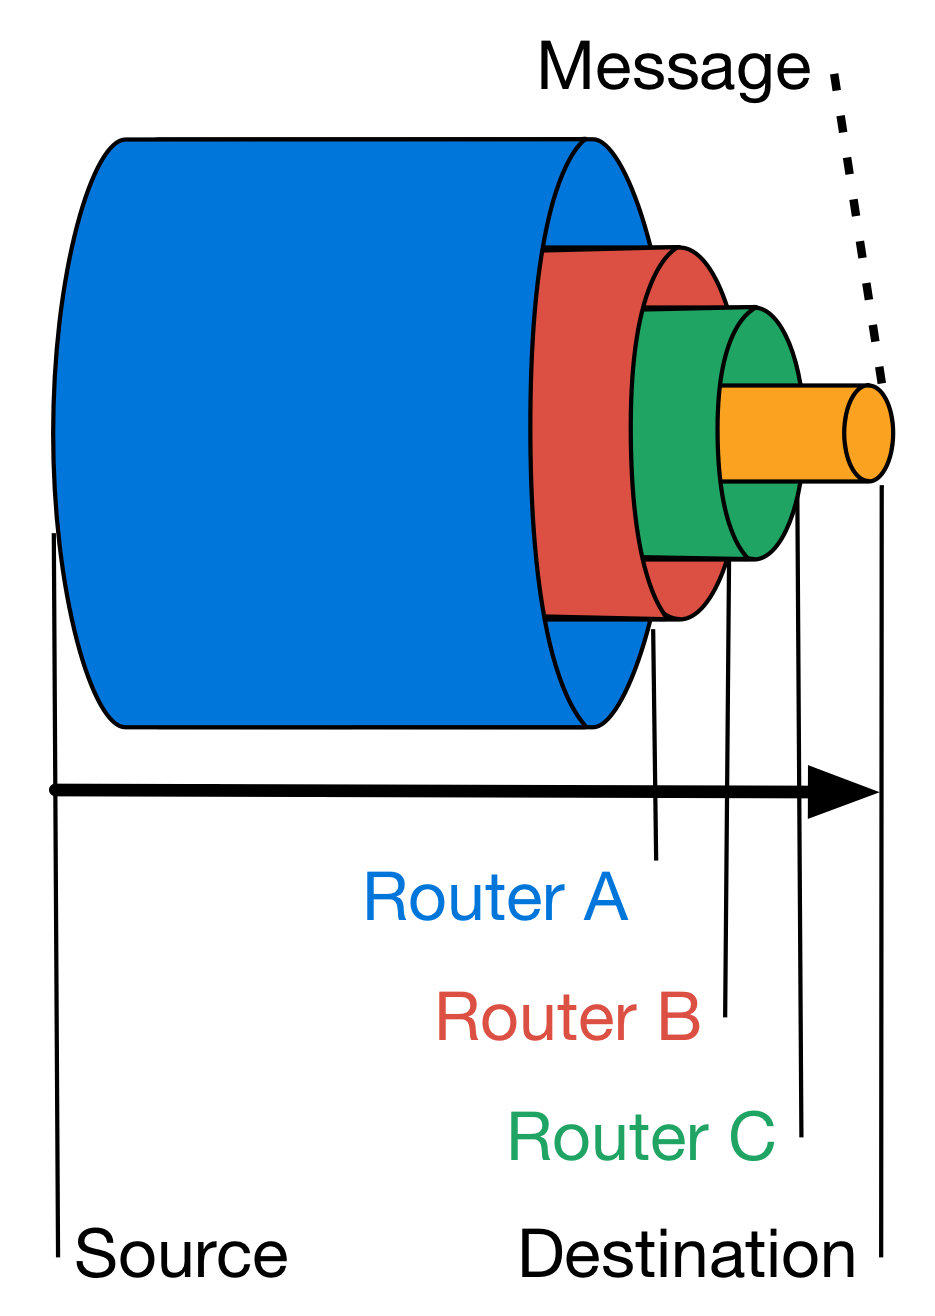
\includegraphics[width=\marginparwidth]{images/onion}
\caption[Tor Onion Encryption]{In this example, the message is sequentially encrypted with keys from router C, B, and A. It is then routed through these routers starting from A. Each router removes a layer of encryption and routes the message to the next router. Finally, router C transmits the message to the destination. This example is taken from \protect\url{wikipedia.org}.}
\label{fig:onion}
}

In order to establish a communication through Tor, a client randomly chooses nodes to build a routing circuit.
In a circuit, each node knows only the previous and next nodes.
The entry node (resp. the exit node) knows only the IP of the source client (resp. the destination client).
Before sending a packet to the circuit the client encrypts it sequentially with the public key of each nodes part of the circuit, starting from the exit node.
This creates layers of encryption around the original packet.
To route a Tor packet, each node decrypts the received packet using its own private key, peeling an encryption layer each time.
The resulting packet is then sent to the next node in the circuit.
When the exit node finally decrypts the packet the original \gls{tcp} packet is recovered and sent in clear to its destination.
An example of onion routing is presented in Figure~\ref{fig:onion}.


Tor is particularly useful for avoiding traffic analysis and circumventing internet censorship.
This is particularly of interest for journalists, human-rights activists, lawyer, and whistleblowers.
However, due to the time consuming layered encryption of each packet and the additional routing overhead, the latency over the Tor network is quite high compared to the standard Internet.
Additionally, some JavaScript functionalities or other libraries can reveal privacy-sensitive data.
As a result, they are blocked by Tor Browser.
For these reasons Tor is not adapted to protect web real-time media communications and WebRTC is actually not implemented in the Tor Browser.


%%%%%%%%%%%%%%%%%%%%%%%%%%%%%%%%%%%%%%%%%%%%%%%%%%%%%%
%%%%%%        SIGNALLING ARCHITECTURE
%%%%%%%%%%%%%%%%%%%%%%%%%%%%%%%%%%%%%%%%%%%%%%%%%%%%%%
\section{Signalling Architectures}
\label{sec:voip}

WebRTC does not mandate any signalling architectures.
Silo architectures are the most frequent for web services but do not offer interoperability between \gls{cs}.
In this configuration users are captive of their \gls{cs} domain.
This architecture can be represented in a triangle involving only one \gls{cs} server, as in Figure~\ref{fig:silo}, 
On the contrary, interoperable architectures allow users of some \gls{cs} to call users from other \gls{cs}. 
They are often represented as a trapezoid architecture with the signalling path involving two \gls{cs} servers as in Figure~\ref{fig:webrtcsig}.

\begin{figure}
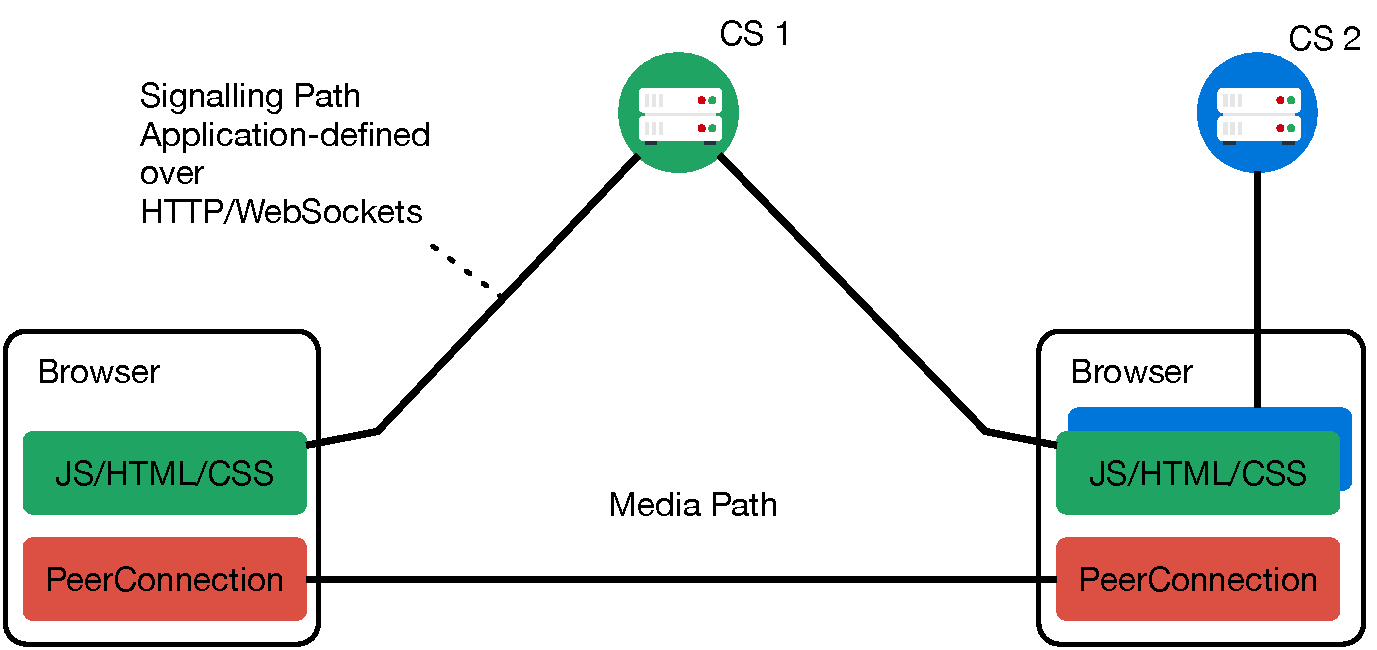
\includegraphics[width=.8\textwidth]{images/silo}
\caption[Silo Architecture]{In silo architecture users have to connect though the same \gls{cs} to establish a session.}
\label{fig:silo}
\end{figure}

Many existing companies offer \gls{voip} communication services, some of which are already switching to WebRTC\footnote{Interestingly, browsers makers porting their own communication services to WebRTC aim first at compatibility with their existing solutions and tend to implement non-standard features in their WebRTC implementation. For instance, WebRTC in Chrome supports \gls{sdes} to cater for hangouts while Edge's first video codec support was H.264 Skype's proprietary codec.}.
The only constraint for signalling is that it uses the \gls{sdp} offer/answer model.
For the moment \gls{voip} communication services on the Web are heavily relying on the silo model.
More complex architectures are being developed to allow inter-domain interoperability.
These architectures differ by the way they handle user discovery, routing, and identity management and formats.
Although the main use case for WebRTC is \gls{voip}, other services such as video streaming~\cite{nurminen2013p2p} and data sharing~\cite{vogt2013leveraging} can be supported.
In this section, we give a quick overview of some interoperable and distributed signalling architectures.

\subsection{Voice over LTE and WebRTC Interconnectivity}
\label{sec:ims}
\gls{volte} is an architecture for \gls{voip} over 4G mobile networks.
Figure~\ref{fig:volte} presents a simplified view of the \gls{lte} mobile network, a standard for high-speed mobile networks designed by the \gls{3gpp}.
This architecture is separated in an access network, \ie a network of eNodeB responsible for all radio-related functions including encryption of data sent over radio interfaces, and a core network responsible for the control of the \gls{ue} and the establishment of \gls{ip} connectivity.
In the core network, the Serving Gateway (S-GW) and Mobility Management Entity (MME) handle the \gls{ue} mobility, while the PDN Gateway (P-GW) handles \gls{ip} addresses allocation and \gls{qos} enforcement.
Finally, the Home Subscriber Server (HSS) is a database containing user's profile, location, and IP information.
It is responsible for the user authentication, subscription, and discovery.
\gls{volte} interconnects the \gls{lte} network with the \gls{ims} network.
The main goal of the \gls{ims} is to achieve the concept of Fixed Mobile Convergence\footnote{The convergence of fixed and mobile telephony networks under an All-\gls{ip} environment.}.
A simplified view of the \gls{ims} architecture is presented in Figure~\ref{fig:ims}.
\gls{cscf} form the core of an IMS domain.
The Proxy-\gls{cscf} (P-CSCF) is a \gls{sip} proxy server which serves as the point of contact for each user equipment.
When a \gls{ue} connects to a network, it looks up for a reachable P-\gls{cscf}.
In \gls{ims} roaming scenario, the \gls{ue} connects directly to the visited network's P-\gls{cscf} rather than to his home network. 

\begin{figure}[tbp]
\begin{center}
\begin{subfigure}{\textwidth}
    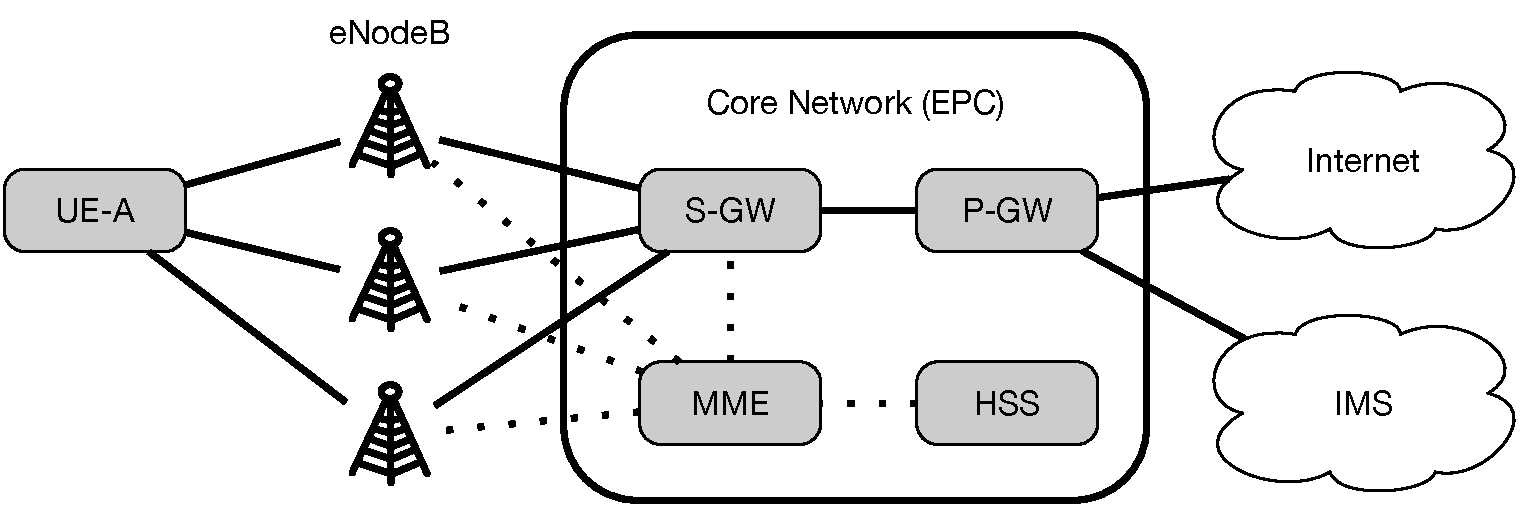
\includegraphics[scale=0.5]{images/VoLTE}
\caption{Simplified LTE architecture.}
\label{fig:volte}
\end{subfigure}\\


\begin{subfigure}{\textwidth}
    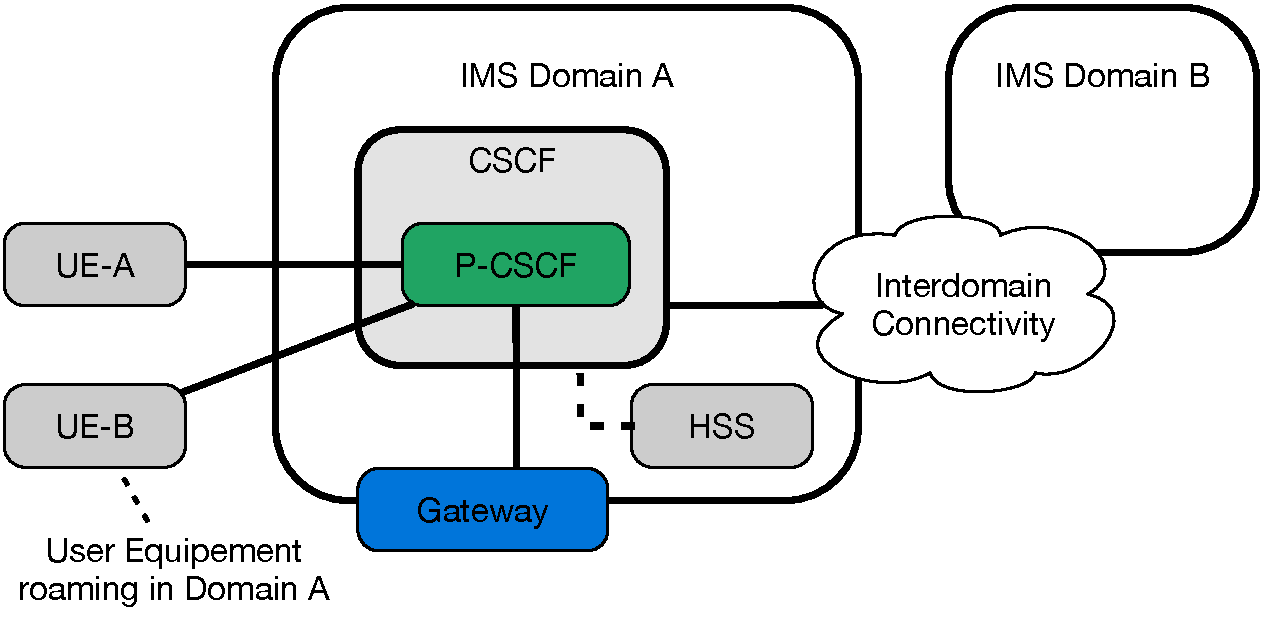
\includegraphics[scale=0.5]{images/IMSArchSimplified}
\caption{Simplified IMS architecture.}
\label{fig:ims}
\end{subfigure}
\caption[Simplified VoLTE Architecture]{A simplified view of the VoLTE architecture. The LTE offers connectivity to the Internet and to the IMS while the IMS offers VoIP service.}
\end{center}
\end{figure}

\gls{sip} is a signalling protocol supporting the determination of user location, availability, as well as session negotiation, setup, and management.
As it is only concerned with the signalling part of the communication session, \gls{sip} is used in conjunction with other protocols such as \gls{sdp} and SRTP (presented in Section~\ref{sec:webrtc}).
A network of proxy servers allows \gls{sip} endpoints to register and routes requests to a user's location.
In \gls{volte}, the \gls{ue} contains a \gls{sip} user-agent and an \gls{uicc} often refered to as a ``SIM Card''.
The \gls{uicc} contains several identity modules including the IP Multimedia Services Identity Module (ISIM) which in particular provides the \gls{ims} home domain name, a private and public identity\footnote{The public identity is a telephone \gls{uri} of the form \texttt{tel:phonenumber}.}, and a secret key used for authentication and registration.

\gls{volte} offers roaming, handover, and interconnectivity with other networks.
Interconnectivity with WebRTC can be handled by an \gls{ims} domain offering a compatible gateway (see Figure~\ref{fig:ims}).
In this case, the \gls{ims} domain has to deploy a WebRTC web server, a WebRTC JavaScript client, and enhanced functionalities for WebRTC in the P-\gls{cscf}.
The gateway performs adaptation between WebRTC and \gls{ims} protocols such as transcoding and encryption.
While encryption using \gls{dtlssrtp} is mandatory in WebRTC (see Section~\ref{sec:webrtcid}), encryption of both media and signalling is optional in the \gls{ims}.
Furthermore, as \gls{volte} security relies on the radio encryption of the access network, its \gls{rtp} profile does not support encryption.
This constraint implies that WebRTC-\gls{volte} interconnectivity cannot use End-to-End encryption with \gls{srtp} and is instead limited to End-to-Access-Edge encryption (see Figure~\ref{fig:voltesecurity}).

\begin{figure}[tbp]
\begin{center}
\begin{subfigure}{\textwidth}
    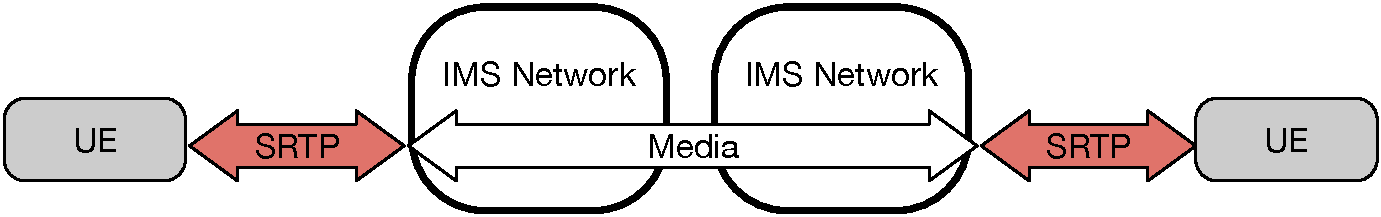
\includegraphics[scale=0.5]{images/e2aeEncryption}
\caption{End-to-Access-Edge Encryption}
\label{fig:e2ae}
\end{subfigure}\\


\begin{subfigure}{\textwidth}
    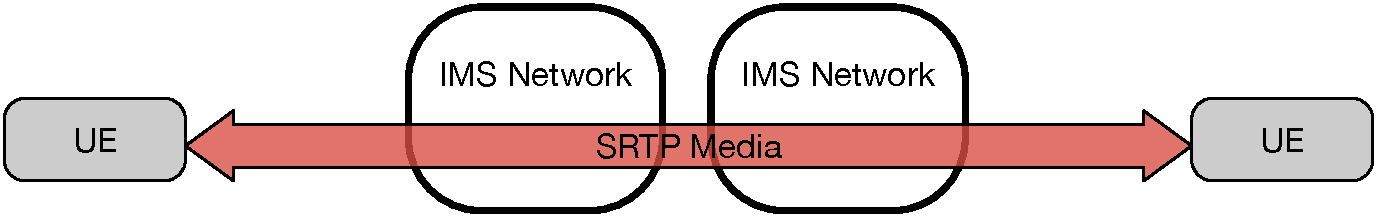
\includegraphics[scale=0.5]{images/e2eEncryption}
\caption{End-to-End Encryption.}
\label{fig:e2e}
\end{subfigure}
\caption[E2E and E2AE IMS Encryption]{End-to-End and End-to-Access-Edge encryption scenario over IMS networks.}
\label{fig:voltesecurity}
\end{center}
\end{figure}


\subsection{Matrix}
\label{sec:matrix}

Matrix~\cite{matrix} is a specification for a messaging and data synchronisation federation.
One of its use cases is the exchange of signalling message for WebRTC communications.
Figure~\ref{fig:matrix} shows three users, each connected to a Matrix home server, and exchanging synchronised message in a room. 

Matrix specifies several \gls{api}, amongst which a client-server and a server-server \gls{api}.
The server-server \gls{api} defines the \gls{http} interfaces and data format allowing Matrix home servers to synchronise messages with each other in real-time.
Servers can either push a message to another server, broadcast it to all servers in a room, or make a query to a server to get a state snapshot.
This \gls{api} also defines how servers are discovered and authenticated, and how user's presence information is exchanged between home servers.
The client-server \gls{api} defines the \gls{http} interfaces for a client application to connect and communicate with a Matrix home server.
It allows the application to manage rooms and send messages.
The client-server \gls{api} also defines how users authenticate to their home server through any Matrix application.
This particularity of the Matrix architecture means that users can choose any application to connect to any home server.

Matrix user identifiers are of the form \texttt{@UserID:HomeServerDomain}.
These identifiers are used internally by home servers, and in particular for home server discovery.
However, Matrix also defines third-party identifiers (3PID) as a more user-friendly way to refer to users.
The Identity Service \gls{api} defines how 3PID are associated to Matrix identifiers, stored, and queried.
This service relies on a trusted federation of Matrix identity servers.

Despite its interesting concepts, the Matrix ecosystem is still in early development.
Most implementations are in the alpha stage and the specification itself is rated as unstable.
The Matrix identity specification is the less advanced specification, and no identity server implementation is referenced on the Matrix webpage. 

\begin{figure}
\begin{center}
    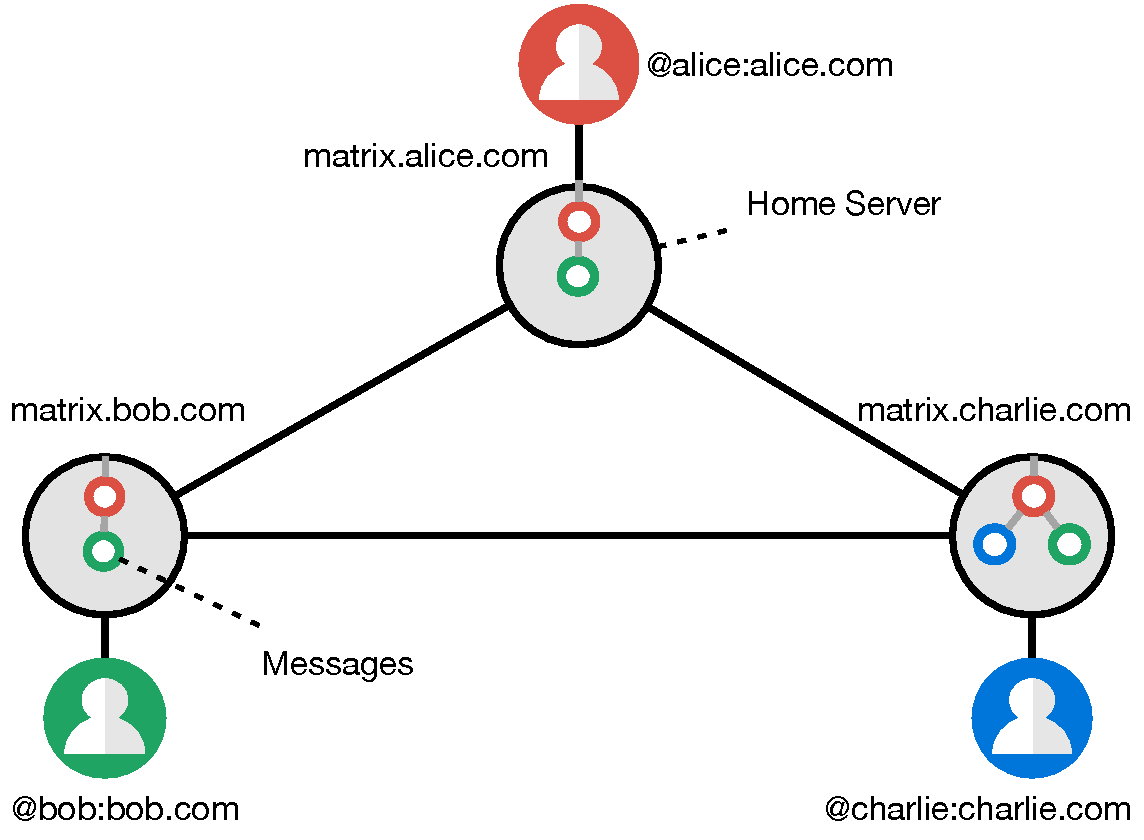
\includegraphics[scale=0.5]{images/matrixArch}
\end{center}
\caption[Matrix Messaging Federation]{Federated messaging and data synchronisation between three Matrix home servers.}
\label{fig:matrix}
\end{figure}

\subsection{reThink}
\label{sec:rethink}

reThink, an H2020 European project, specified and experimented with a real-time communication framework.
Its global objective is to allow Telcos to compete with large \gls{ott} companies by offering open and interoperable communication services and applications.

A simplified view of the reThink architecture is presented in Figure~\ref{fig:rethinkArch}.
It builds on the earlier signalling on-the-fly concept from the Wonder European project\footnote{\url{http://hypercomm.github.io/wonder/}}.
Signalling on-the-fly avoids the standardisation of messaging protocols by providing a messaging \gls{api}.
When two parties want to communicate, they agree on a protocol and download the corresponding protocol-stub implementing the messaging \gls{api}.
While this architecture allows interoperability without standards protocols, it still requires standardisation of the messaging \gls{api} and message format used for communication.

On the user's side, reThink applications are executed inside the runtime.
The runtime can be a modified web browser or a native program\footnote{The runtime was initially envisioned as a web browser modification. However, it was implemented as a JavaScript library due to the complexity and costs involved.}.
reThink applications make use of modular software components, called hyperties.
These hyperties are downloaded from service provider catalogues and executed in sandboxed environments.
Hyperties can provide many services to an application, including \gls{p2p} communications.
In the interoperable reThink architecture, users can connect to each other through different service providers.
Signalling between two hyperties is thus established through one users' service provider.
More specifically through a messaging node exposed by the selected service provider. 
In order to establish the connection, both runtimes agree on available protocols and download the corresponding proto-stub from the chosen service provider's catalogue.
This process allows hyperties to set up their session and eventually open a \gls{p2p} communication.

\begin{figure*}[tbp]
\begin{center}
    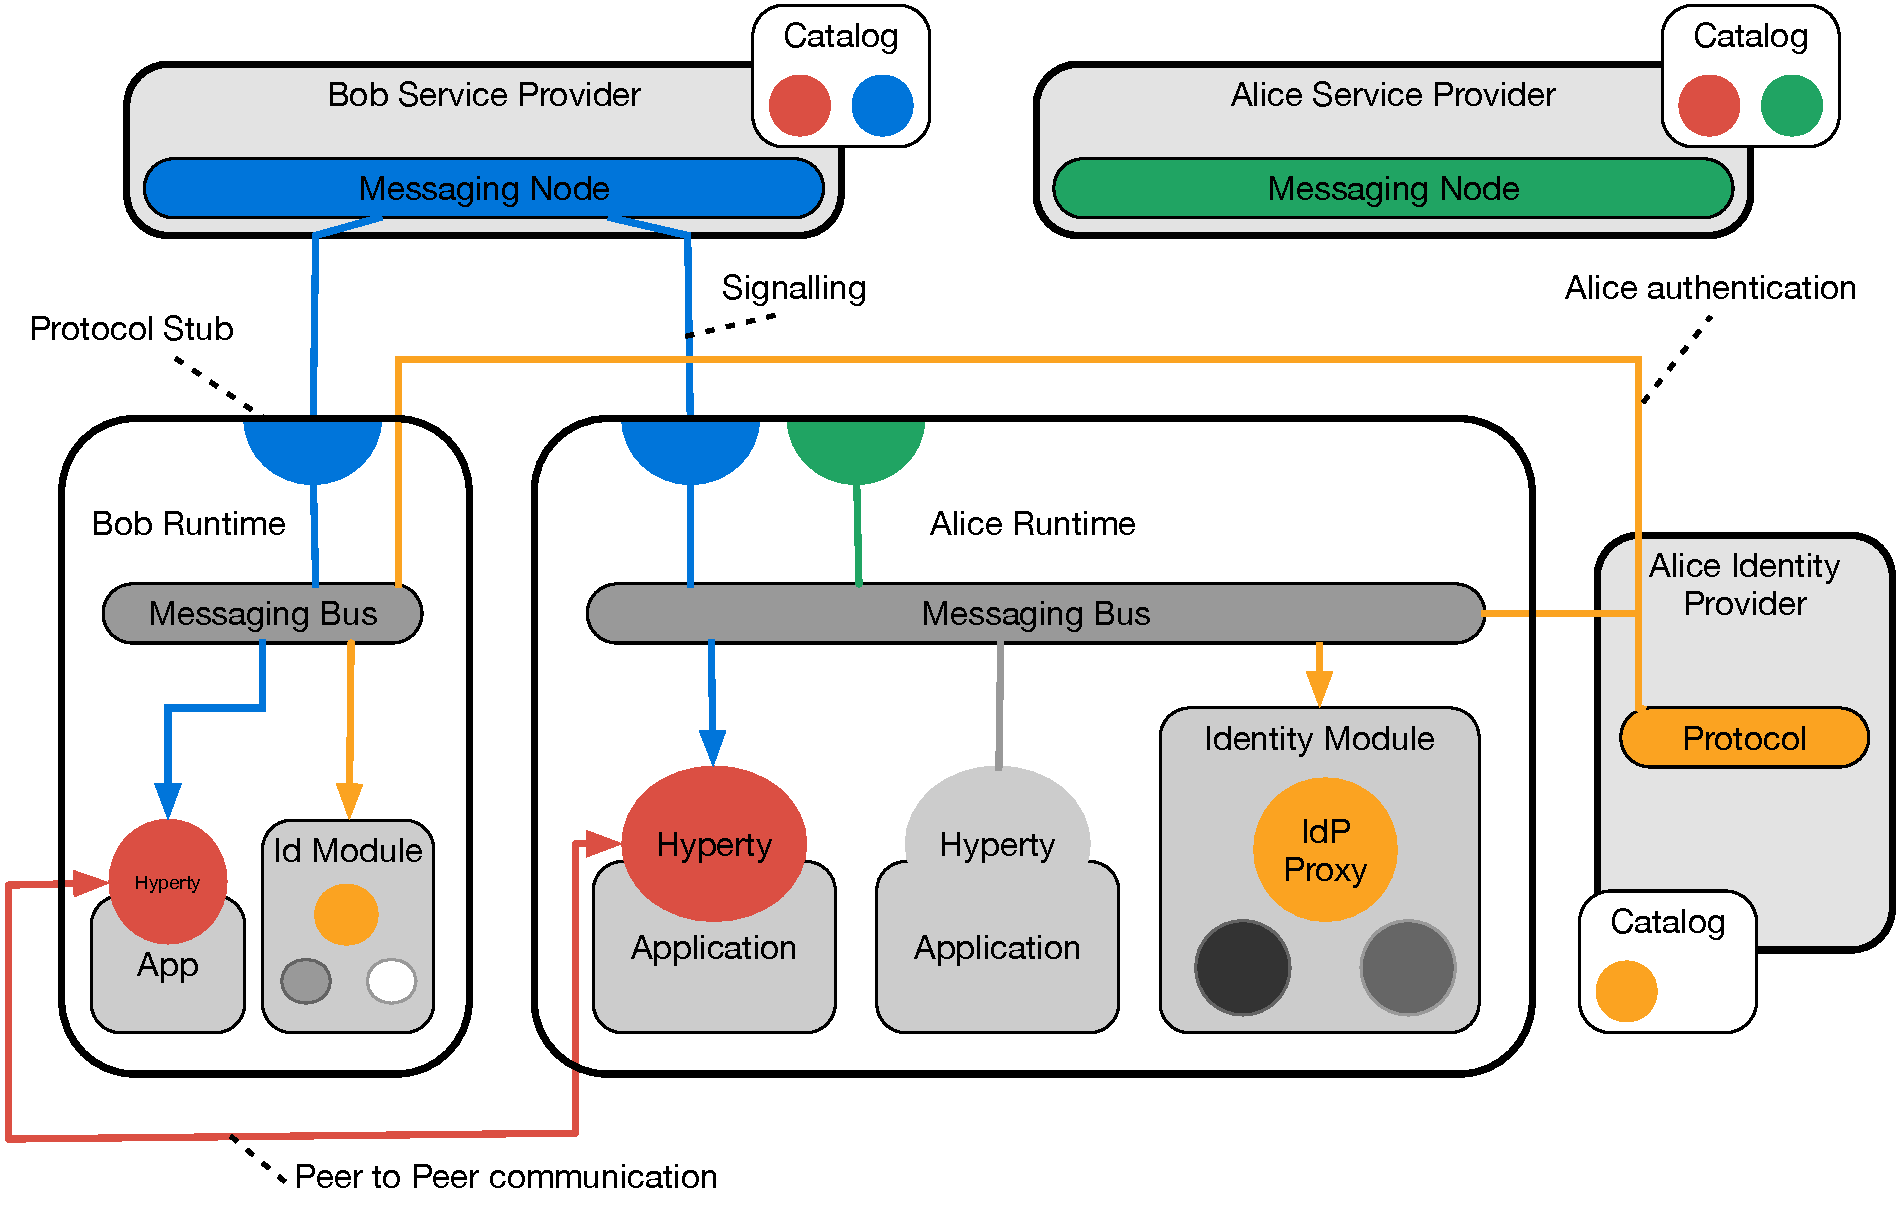
\includegraphics[scale=0.45]{images/rethinkArch}
\end{center}
\caption{Simplified reThink architecture}
\label{fig:rethinkArch}
\end{figure*}

Identity management in the reThink architecture is handled by the Identity Module and reuses the concept of the WebRTC \gls{idp} Proxy.
Some of its design objectives in addition to the WebRTC compatibility are the ability for users to choose their \gls{idp} and the availability of discovery and presence services.
In particular, reThink discovery, presented in Figure~\ref{fig:rethinkDiscovery}, is a layered architecture relying on a cryptographic \gls{guid}.
The global registry, a trusted distributed hash table run by a consortium of service providers, maps \gls{guid} to user profile information.
Users can manage and control their public profile information stored in the \gls{dht} by proving ownership of a private key.
These user profiles also point to user identities on service providers by exposing pairs of service provider domain and service bound user identifiers.
Services providers, in turn, expose a domain registry containing the user's reachability information.
\gls{guid} can either be exchanged manually or discovered through the use of a discovery service.

%reThink identity design objectives are WebRTC compatibility, \ie IdP exposing a WebRTC \gls{idp} Proxy would be also compatible with reThink, and .
\begin{figure}
\begin{center}
    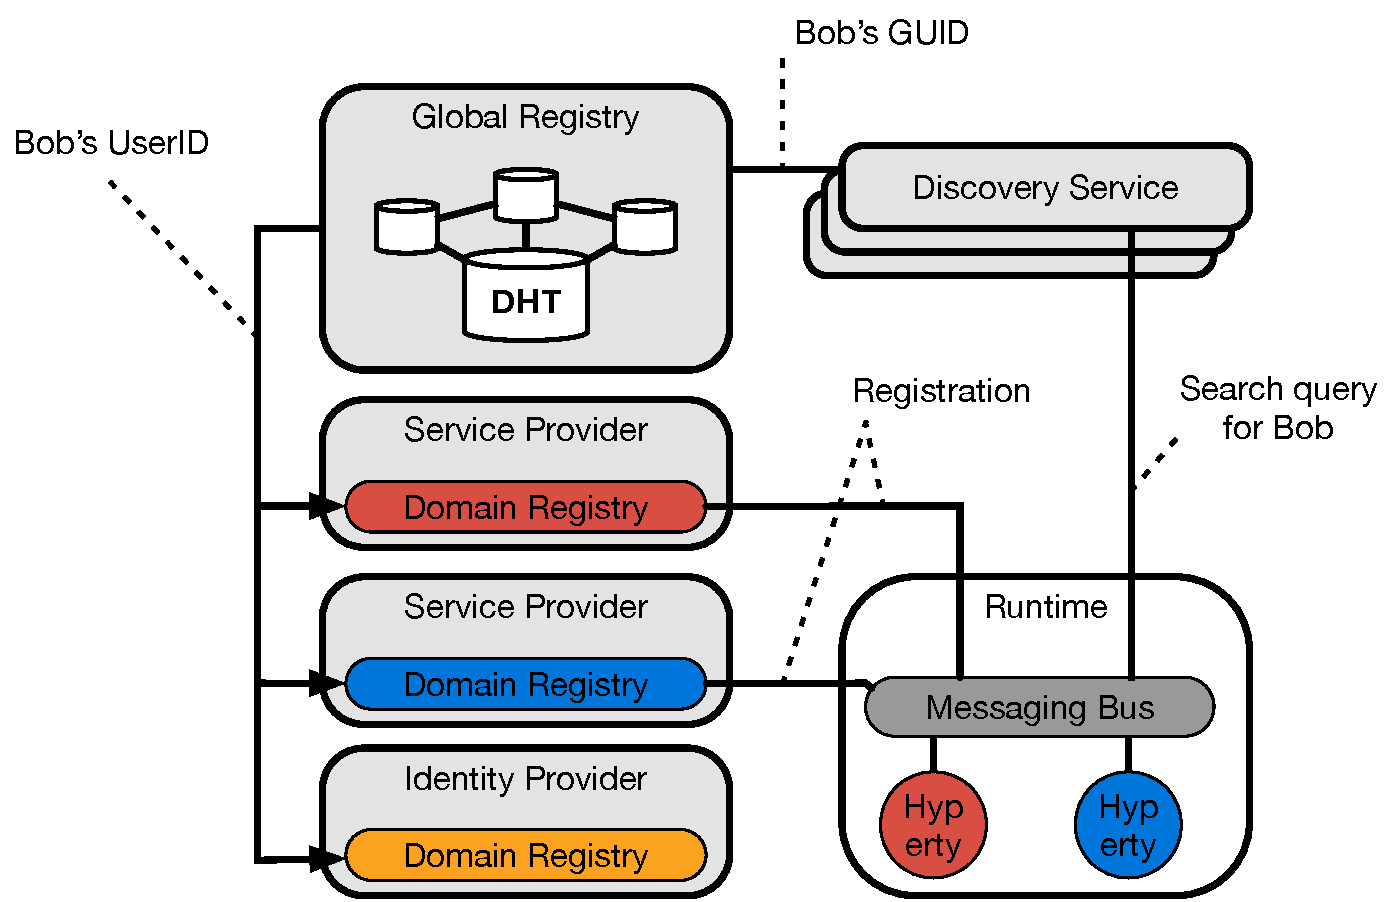
\includegraphics[scale=0.5]{images/rethinkDiscovery}
\end{center}
\caption{reThink Identity Discovery}
\label{fig:rethinkDiscovery}
\end{figure}



\subsection{Distributed Signalling Architectures}
\label{sec:spray}
The rapid growth of web traffic and video streaming, in particular, has an important impact on infrastructure costs both for content providers and network operators.
\gls{cdn} are constituted of proxy servers geographically distributed to be as close to clients as possible.
Besides tidying core network traffic, \gls{cdn} optimise the availability and performance of content delivery through various techniques and in particular caching, load-balancing, and routing techniques.
Distributed \gls{cdn} merge the advantages of \gls{cdn} and \gls{p2p} networks.
These networks leverage their clients' upload bandwidth to redistribute content to other clients and further reduce costs.
However, distributed \gls{cdn} require the installation of client-side software or browser plugin~\cite{roverso2014hive}.

WebRTC allows browser-to-browser \gls{p2p} communication for video streaming and data channels without third-party plugins.
It is thus possible to build distributed \gls{cdn} around a network of WebRTC enabled browser.
To create such network, clients first reach a bootstrapping server.
This server allows new clients to open data channels with other clients already part of the network.
These data channels form an overlay signalling network.
Once a client joined the network, it can discover other distant clients and establish \gls{p2p} connections with them, for instance, to retrieve a file or a video stream. 
Figure~\ref{fig:spray} shows an example of such network architecture where P3 joins the network and finally retrieves a video stream from P1.
As the signalling message from P3 to P1 goes through P2, the signalling architecture is similar to \gls{mitm} attack as shown in Figure~\ref{fig:mitm}.
Such signalling path may not be trusted and depending on the use case it may be an issue.
Zhang~\etal\cite{zhang2013maygh} also report some security and privacy considerations for their WebRTC \gls{cdn} framework.

\begin{figure}
\begin{center}
    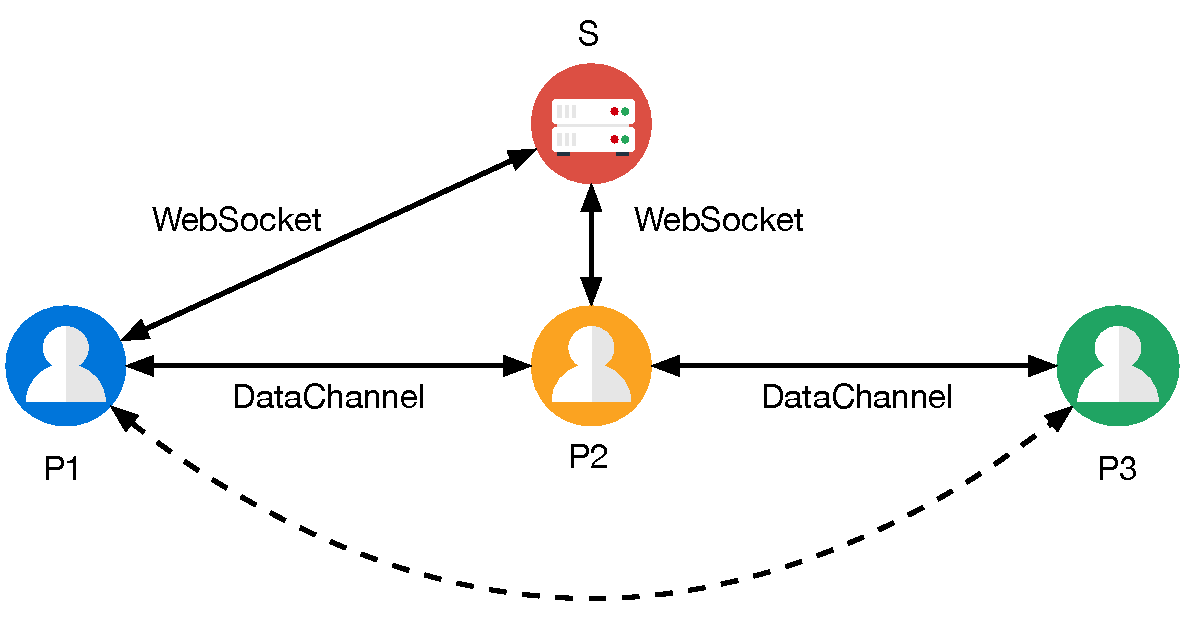
\includegraphics[scale=0.5]{images/sprayArch}
\end{center}
\caption[Spray Architecture]{In this example P1 and P2 are already part of the network. To join the network P3 first reaches the bootstrapping server S.
S signals P2 and P3 so that they open a P2P data channel. P3 then requests a video stream from P1. \gls{sdp} messages between P3 and P1 are signalled through P2 using existing data channels. Finally, the video stream is established from P1 to P3~\cite{nedelec2015spray}.}
\label{fig:spray}
\end{figure}


\clearpage
\invisiblesection{Summary}
\label{sec:contextSummary}
%\vspace*{3cm}

\blockmargin%
%\hspace{-\marginparwidth}\hspace{-\marginparsep}
\makebox[\overflowingheadlen][l]{
\begin{minipage}{\overflowingheadlen}

\begin{mdframed}[style=ContextFrame,frametitle={\ref{sec:contextSummary}~Summary}]
The WebRTC peer-to-peer media path is negotiated by peers exchanging \gls{sdp} offer/answer messages over the signalling path.
Media path encryption is mandatory and is mainly built around the \gls{dtls} and \gls{srtp} protocols. 
It ensures confidentiality and integrity of the \gls{p2p} sessions between peers.
The signalling path generally involves one or more signalling server and its security relies on standard web security protocols.
At the root of these protocols is the web browser which acts as the trusted computing base.
WebRTC applications and their associated signalling servers are also responsible to protect the availability of the session and network resources by filtering incoming call.

\medskip

Depending on the signalling architecture or the signalling servers' origin the signalling path may be untrusted by users.
WebRTC remedies to this issue by allowing peers to bind \gls{dtls} certificates to identity assertions.
These assertions are generated and verified by identity providers forming two symmetric identity paths.
Paradoxically, these identity paths are configured by the communication services.

\medskip

Privacy is a growing concern for users and contributors of web specifications alike.
The main privacy threats against WebRTC users are related to identification of anonymous callers and correlation of web browsing and call history.
Browsers enforce consent policies to protect users against malicious sites launching non-legitimate calls.
However, legitimate communication services also gain an important knowledge of their users' call history.

\medskip



\end{mdframed}

\end{minipage}
}
\unblockmargin

%
%
%\todo{Should we conclude the summary by a reference to the research questions? Given the responsibility of actors of the call setup related to the security and privacy of WebRTC communications, users should be able to choose trusted actors and understand to which level is their security guaranteed. At the moment, the WebRTC trust model is quite informal. and so on.}
